% CSAD-AT 小论文 - 《数据与计算发展前沿》投稿格式
% 三线表 + 中英文双语标题
\documentclass[10.5pt,a4paper,twocolumn]{ctexart}

% ==================== 宏包 ====================
\usepackage[left=2cm,right=2cm,top=2.5cm,bottom=2.5cm]{geometry}
\usepackage{graphicx}
\usepackage{booktabs}       % 三线表
\usepackage{multirow}
\usepackage{amsmath,amssymb}
\usepackage{algorithm}
\usepackage{algorithmic}
\usepackage[hidelinks]{hyperref}
\usepackage{cite}
\usepackage{caption}
\usepackage{subcaption}
\usepackage{enumitem}
\usepackage{url}
\usepackage{xcolor}
\usepackage{float}

% ==================== 格式设置 ====================
\setlength{\columnsep}{0.7cm}
\renewcommand{\abstractname}{}
\CTEXsetup[format={\bfseries\zihao{4}}]{section}
\CTEXsetup[format={\bfseries\zihao{5}}]{subsection}
\CTEXsetup[format={\bfseries\zihao{5}}]{subsubsection}
\captionsetup{font=small,labelsep=space}
\captionsetup[table]{position=top}
\captionsetup[figure]{position=bottom}

% 图片路径
\graphicspath{{Img/}{Tex/}}

% ==================== 自定义双语标题命令 ====================
\newcommand{\bicaption}[2]{%
  \caption{#1\\{\small #2}}%
}

% ==================== 文档开始 ====================
\begin{document}

% ==================== 标题区（单栏） ====================
\twocolumn[
\begin{@twocolumnfalse}
\begin{center}

{\zihao{2}\bfseries CSAD-AT：面向分布式集群的阈值自适应\\单指标多节点异常检测框架\par}
\vspace{0.8em}

{\zihao{5} 杨婧雯$^{1}$，裴昌华$^{1*}$\par}
\vspace{0.3em}
{\zihao{6} 1.~中国科学院计算机网络信息中心，北京~~100190\par}
\vspace{1em}

% ---------- 中文摘要 ----------
\parbox{0.92\textwidth}{\zihao{5}
\textbf{摘\quad 要：}【目的】分布式集群中负载均衡类监控指标的正常波动具有随机性和不可预测性，传统基于历史模式学习的异常检测方法难以适用。同时，基于节点曲线相似性的检测方法对阈值参数高度敏感，难以在生产环境中直接部署。本文旨在提出一种无需人工阈值调优的端到端自适应异常检测框架。【方法】本文提出CSAD-AT（Curve Similarity-based Anomaly Detection with Adaptive Threshold）框架，融合欧氏距离、自编码器嵌入和局部密度偏离三种互补的曲线相似性评分方法，通过MinMax归一化与加权聚合统一多视角分数，并提出I-SPOT自适应阈值算法，采用包容性数据池更新与周期性GPD重估机制动态确定异常判定边界。【结果】在基于中国联通大数据生产环境构建的单指标多节点数据集上，CSAD-AT在无需人工阈值调整的条件下取得了0.9864的F1分数，优于三种曲线相似性方法在最优人工调参下的表现，且显著优于六种主流多元时序异常检测基线算法。【局限】当前实验仅在单一监控指标（RPC连接数）上验证，尚未扩展至多指标联合检测场景。【结论】基于节点曲线相似性的检测思路能够有效应对负载均衡类指标的随机波动挑战，I-SPOT自适应阈值算法成功消除了人工调参依赖，CSAD-AT框架具有良好的实际部署价值。
}
\vspace{0.4em}

\parbox{0.92\textwidth}{\zihao{5}
\textbf{关键词：}异常检测；分布式集群；曲线相似性；自适应阈值；极值理论
}
\vspace{1.2em}

% ---------- 英文标题 ----------
{\zihao{4}\bfseries CSAD-AT: A Threshold-Adaptive Single-Metric Multi-Node\\ Anomaly Detection Framework for Distributed Clusters\par}
\vspace{0.6em}
{\zihao{5} YANG Jingwen$^{1}$, PEI Changhua$^{1*}$\par}
\vspace{0.3em}
{\zihao{6} 1.~Computer Network Information Center, Chinese Academy of Sciences, Beijing 100190, China\par}
\vspace{0.8em}

% ---------- 英文摘要 ----------
\parbox{0.92\textwidth}{\zihao{5}
\textbf{Abstract:} [Objective] Load-balanced monitoring metrics in distributed clusters exhibit random and unpredictable normal fluctuations, making traditional history-based anomaly detection methods ineffective. While curve similarity-based methods show promise, their high sensitivity to threshold parameters hinders practical deployment. This paper proposes an end-to-end adaptive anomaly detection framework that eliminates manual threshold tuning. [Methods] We propose CSAD-AT (Curve Similarity-based Anomaly Detection with Adaptive Threshold), which integrates three complementary scoring methods based on Euclidean distance, autoencoder embedding, and local density deviation. Scores are unified through MinMax normalization and weighted aggregation. An improved I-SPOT adaptive threshold algorithm with inclusive data pool updates and periodic GPD re-estimation dynamically determines anomaly boundaries. [Results] On a single-metric multi-node dataset from China Unicom production environments, CSAD-AT achieves an F1 score of 0.9864 without manual threshold tuning, outperforming all three similarity methods under optimal manual tuning and significantly surpassing six state-of-the-art baselines. [Limitations] Experiments are currently limited to a single monitoring metric (RPC connection count). [Conclusions] Curve similarity-based detection effectively addresses the challenge of random fluctuations in load-balanced metrics. The I-SPOT algorithm successfully eliminates manual parameter tuning dependency.
}
\vspace{0.4em}

\parbox{0.92\textwidth}{\zihao{5}
\textbf{Keywords:} anomaly detection; distributed cluster; curve similarity; adaptive threshold; extreme value theory
}
\vspace{1.5em}
\end{center}
\end{@twocolumnfalse}
]


%=====================================================================
%  引言
%=====================================================================
\section{引言}

随着云计算和大数据技术的快速发展，分布式集群已成为支撑大规模数据处理与计算服务的核心基础设施。在企业级生产环境中，分布式集群通常由数十至数百个计算节点组成，通过YARN（Yet Another Resource Negotiator）等资源调度框架实现计算资源的统一管理与动态分配。集群中各节点的运行状态由Prometheus等监控系统持续采集，形成海量的多节点时间序列监控数据。及时准确地从这些监控数据中检测出异常节点，对于保障服务质量、降低运维成本具有重要意义。

然而，分布式集群环境中的异常检测面临独特的技术挑战。以RPC连接数等与用户负载强相关的监控指标为例，其正常波动具有随机性和不可预测性，难以通过先验知识定义统一的正常模式。传统的单节点历史模式学习方法（如基于重构的自编码器、基于预测的Transformer等）在面对此类指标时，往往因无法建立稳定的正常基线而导致高误报率或高漏报率。

值得注意的是，在负载均衡机制的作用下，分布式集群中正常运行的各节点承担相近的工作负载，其同一监控指标的时序曲线呈现出高度的形态相似性。当个别节点发生故障时，其曲线会显著偏离群体模式，形成可识别的"离群曲线"。这一"正常聚集、异常离群"的数据特性为异常检测提供了新思路：通过度量节点间曲线的差异程度来识别偏离群体行为的异常节点。

基于曲线相似性的方法虽然在理论上具有优势，但在实际部署中面临一个核心难题：检测阈值的选择。实验表明，此类方法的最优参数处于极窄的有效区间内，细微的阈值偏移便可导致性能骤变，呈现显著的"悬崖效应"。由于不同集群的节点数量、负载模式、指标量纲等因素各异，在一个集群上调优的参数难以直接迁移，而获取高质量标注数据用于参数调优的成本又极为高昂。因此，如何实现阈值的动态自适应调整，成为将基于曲线相似性的方法推向实际应用的关键技术瓶颈。

针对上述挑战，本文提出CSAD-AT（Curve Similarity-based Anomaly Detection with Adaptive Threshold）框架。该框架融合欧氏距离、自编码器嵌入和局部密度偏离三种互补的曲线相似性评分方法，通过MinMax归一化与加权聚合实现多视角分数融合，并提出I-SPOT（Inclusive SPOT）自适应阈值算法，基于极值理论动态确定异常判定边界，实现端到端的无人工调参异常检测。在基于联通大数据生产环境构建的数据集上，CSAD-AT取得了0.9864的F1分数，显著优于现有基线方法。


%=====================================================================
%  1 相关工作
%=====================================================================
\section{相关工作}

时间序列异常检测是智能运维（AIOps）领域的核心任务之一。现有方法主要包括基于统计的方法、基于机器学习的方法和基于深度学习的方法三大类。

在基于深度学习的方法中，OmniAnomaly\cite{su2019omni}采用随机变分自编码器学习多元时间序列的正常分布，通过重构概率识别异常。USAD\cite{audibert2020usad}在自编码器基础上引入对抗训练增强鲁棒性。TranAD\cite{tuli2022tranad}基于Transformer架构并结合对抗训练提升异常敏感度。GDN\cite{deng2021graph}通过图神经网络建模变量间拓扑关系。MTAD-GAT\cite{zhao2020mtadgat}结合图注意力网络和时间卷积网络同时建模变量间关联和时间依赖。MAD-GAN\cite{li2019madgan}采用LSTM构建生成对抗网络学习正常数据分布。

上述方法主要面向多变量间的关联异常设计，对分布式集群中单指标多节点的场景缺乏针对性。在自适应阈值方面，SPOT算法\cite{siffer2017spot}基于极值理论对流数据进行动态阈值检测，但其排他性更新策略在概念漂移条件下存在阈值衰减问题。本文提出的CSAD-AT框架融合多视角曲线相似性评分与改进的I-SPOT自适应阈值算法，实现端到端的无人工调参异常检测。


%=====================================================================
%  2 数据集构建
%=====================================================================
\section{数据集构建}

\subsection{数据来源与采集}

本研究的数据来源于中国联通大数据生产底座平台。该平台采用YARN架构进行分布式计算资源的统一调度与管理，其核心架构如图\ref{fig:yarn_arch}所示。ResourceManager作为集群的中央调度器，通过RPC Router接收各NodeManager的心跳与资源请求；各NodeManager负责本地容器的生命周期管理，通过RPC Client与ResourceManager保持通信；Prometheus监控系统实时采集各节点的运行指标。

\begin{figure}[htbp]
    \centering
    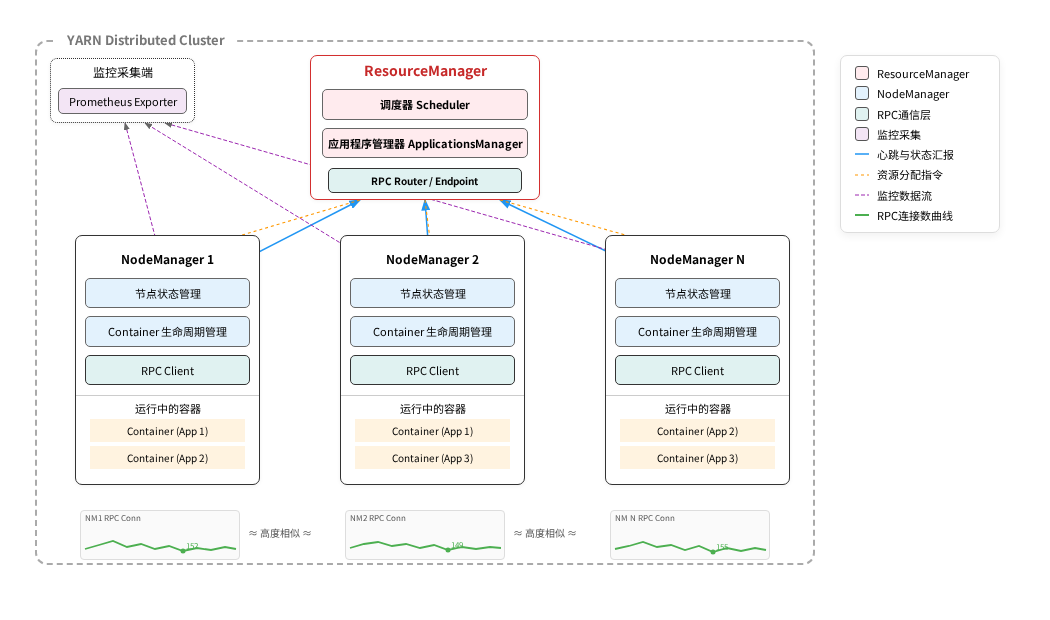
\includegraphics[width=\columnwidth]{yarn_arch.png}
    \bicaption{YARN分布式集群架构与RPC Router连接数指标示意}{YARN cluster architecture and RPC Router connection count}
    \label{fig:yarn_arch}
\end{figure}

在长期运维实践中发现，与用户负载强相关的监控指标（如RPC连接数）呈现出独特的统计特性：正常波动模式难以通过先验知识统一定义，且随全局负载呈现不可预测的剧烈变化。然而，得益于负载均衡机制的作用，正常运行状态下各节点同一指标的时序曲线呈现出高度的形态相似性。本研究选取RPC Router连接数作为核心研究指标，通过Prometheus API接口采集了多个生产集群在连续运行周期内所有节点的该指标时序数据，形成训练集（覆盖30天连续运行数据）和测试集（覆盖8天连续运行数据），原始数据采样间隔为60秒。

\subsection{数据集预处理与标注}

为构建适用于算法研究的高质量数据集，本研究对原始监控时序数据实施了系统化的预处理与半人工标注流程，整体流程如图\ref{fig:annotation_flow}所示。预处理阶段执行三项操作：（1）线性插值填充短暂缺失值；（2）将所有节点数据对齐至统一的60秒间隔时间戳；（3）剔除长时间段数据完全缺失的节点记录。

\begin{figure}[htbp]
    \centering
    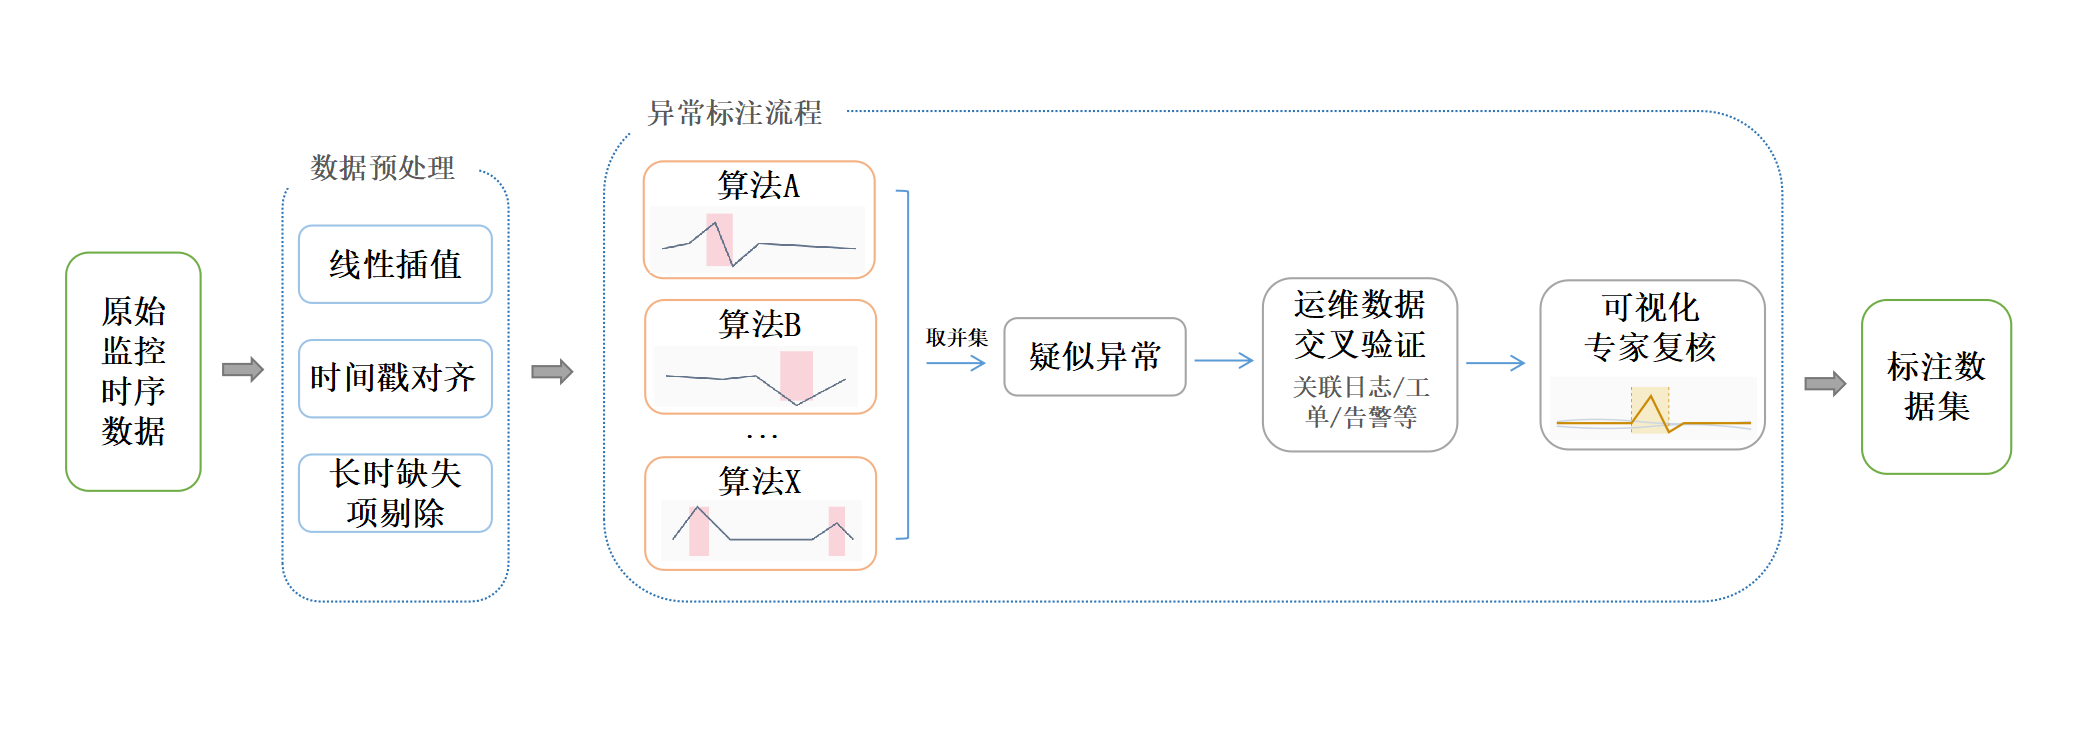
\includegraphics[width=\columnwidth]{draft/annotation_flow_new.png}
    \bicaption{数据集预处理与半人工标注流程}{Dataset preprocessing and semi-manual annotation workflow}
    \label{fig:annotation_flow}
\end{figure}

在异常标注阶段，采用多算法初筛与专家判读相结合的半人工标注策略。首先利用多种无监督离群点检测算法以宽松阈值筛选疑似异常片段；然后关联查询对应节点的运维日志、工单记录等多源数据进行交叉验证；最终由具备丰富运维经验的专家结合可视化工具做出异常判定。

\subsection{数据集统计与可视化}

经过预处理与标注，构建了适用于分布式集群节点级异常检测的单指标多节点时间序列数据集，详细统计信息如表\ref{tab:dataset_stats}所示。

\begin{table}[htbp]
    \centering
    \bicaption{数据集统计数据}{Dataset statistics}
    \label{tab:dataset_stats}
    \begin{tabular}{lccccc}
        \toprule
         & 节点数 & 数据点 & 异常段 & 异常点 & 异常比例 \\
        \midrule
        训练集   & 30 & 86400 & /  & /    & /      \\
        测试集A  & 15 & 11520 & 72 & 901  & 7.82\% \\
        测试集B  & 15 & 11520 & 33 & 907  & 7.87\% \\
        测试集   & 30 & 23040 & 105& 1808 & 7.85\% \\
        \bottomrule
    \end{tabular}
\end{table}

该数据集的核心特征在于直观揭示了分布式集群在负载均衡机制下的运行规律，如图\ref{fig:anomaly_curve}所示。在绝大部分时间内，集群内多数节点的监控指标曲线呈现高度的形态同步性与数值聚集性，形成清晰的"正常行为簇"。当个别节点发生故障时，其曲线显著偏离共同的"行为簇"，表现为"离群曲线"。

\begin{figure}[htbp]
    \centering
    
\includegraphics[width=\columnwidth]{dataset_anomaly_example.png}
    \bicaption{测试集A典型异常片段时序可视化（红色曲线为异常节点，粉色阴影为异常时段）}{Visualization of typical anomaly segments in Test Set A}
    \label{fig:anomaly_curve}
\end{figure}


%=====================================================================
%  3 基于曲线相似性的异常评分方法
%=====================================================================
\section{基于曲线相似性的异常评分方法}

本节从数值距离、嵌入空间距离和局部密度三个互补视角设计异常评分方法。三种方法的核心思想一致：通过度量节点间曲线的偏离程度量化异常可能性。

\subsection{基于欧氏距离的数值相似性度量}\label{subsec:euclidean}

给定包含$N$个节点的分布式集群，每个节点$i$在时刻$t$的监控指标观测值记为$x_i^t$。采用滑动窗口机制对原始序列进行分段处理，对于长度为$w$的时间窗口，节点$i$在时刻$t$的窗口序列表示为$\mathbf{x}_i^t = [x_i^{t-w+1}, \ldots, x_i^t]^T \in \mathbb{R}^w$。节点$i$与节点$j$在时刻$t$的欧氏距离定义为：
\begin{equation}
    d_{ij}^t = \|\mathbf{x}_i^t - \mathbf{x}_j^t\|_2 = \sqrt{\sum_{k=t-w+1}^{t}(x_i^k - x_j^k)^2}
\end{equation}

计算所有节点两两之间的欧氏距离构成距离矩阵$\mathbf{D}^t \in \mathbb{R}^{N \times N}$，计算均值$\mu_t$和标准差$\sigma_t$。对每个节点$i$，计算其与其他所有节点的平均距离：
\begin{equation}
    \bar{d}_i^t = \frac{1}{N-1}\sum_{j=1, j \neq i}^{N} d_{ij}^t
\end{equation}

节点$i$的异常分数采用Z-score标准化形式：
\begin{equation}\label{eq:euc_score}
    s_i^t = \frac{\bar{d}_i^t - \mu_t}{\sigma_t}
\end{equation}

设定阈值$T$，若$s_i^t > T$则判定节点$i$在时刻$t$异常。

\subsection{基于自编码器嵌入的形态相似性度量}

欧氏距离方法对曲线绝对数值高度敏感，可能忽略形态层面的相似性。为克服此局限，引入自编码器进行深度特征提取，其网络结构如图\ref{fig:autoencoder}所示。

\begin{figure}[htbp]
    \centering
    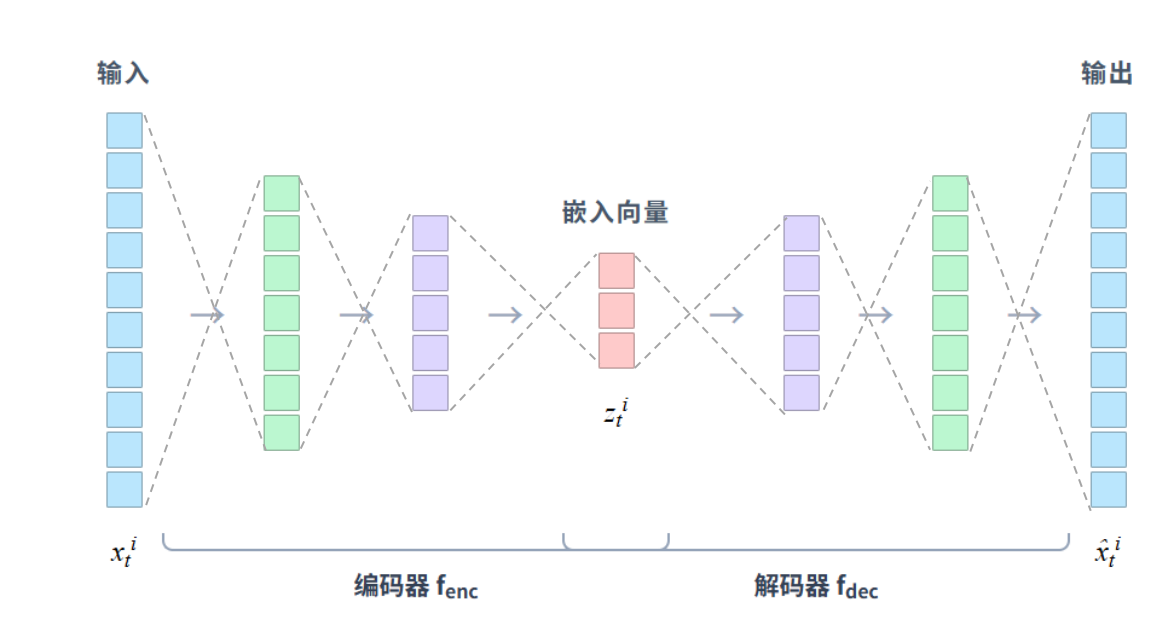
\includegraphics[width=0.85\columnwidth]{draft/autoencoder_arch.png}
    \bicaption{自编码器网络结构示意图}{Architecture of the autoencoder network}
    \label{fig:autoencoder}
\end{figure}

编码器$f_{\text{enc}}$通过多层全连接网络将输入序列$\mathbf{x}_i^t$压缩为低维嵌入向量$\mathbf{z}_i^t = f_{\text{enc}}(\mathbf{x}_i^t)$，解码器$f_{\text{dec}}$以对称结构重构原始输入$\hat{\mathbf{x}}_i^t = f_{\text{dec}}(\mathbf{z}_i^t)$。通过最小化均方误差训练，嵌入向量保留曲线最本质的形态特征。网络包含三层全连接编码器（维度$w \to 128 \to 128 \to 5$）和对称的三层解码器，隐藏层采用ReLU激活函数，Adam优化器，学习率0.001，训练50个epoch。应用阶段仅使用编码器，基于嵌入向量计算节点间距离$d_{ij}^t = \|\mathbf{z}_i^t - \mathbf{z}_j^t\|_2$，后续异常分数计算与欧氏距离方法一致。

\subsection{基于局部密度的偏离评分}\label{subsec:density}

借鉴局部离群因子（LOF）的思想，设计基于$k$近邻可达密度的连续异常评分方法。对每个时间窗口内的每个节点$i$，基于距离矩阵找到其$k_{\text{nn}}$个最近邻节点，计算局部可达密度：
\begin{equation}
    \text{LRD}_i = \frac{1}{\frac{1}{|\mathcal{N}_i|}\sum_{j \in \mathcal{N}_i} d_{ij} + \epsilon}
\end{equation}
其中$\mathcal{N}_i$为节点$i$的邻域集合，$\epsilon$为防止除零的小常数。密度偏离分数通过三个子分数的加权组合得到：
\begin{equation}\label{eq:density_score}
    s_i^t = w_1 \cdot z_{\text{LRD}} + w_2 \cdot z_{k\text{th}} + w_3 \cdot z_{\text{nbr}}
\end{equation}
其中$z_{\text{LRD}}$、$z_{k\text{th}}$、$z_{\text{nbr}}$分别为LRD、第$k$近邻距离和邻居数量的Z-score标准化值。

\subsection{参数敏感性分析}\label{subsec:sensitivity}

在构建的数据集上进行实验评估，三种方法在最优参数下的检测结果如表\ref{tab:baseline_results}所示，F1分数均超过0.96，显著优于现有基线算法。

\begin{table*}[htbp]
    \centering
    \bicaption{基线算法与曲线相似性方法异常检测结果}{Anomaly detection results of baseline algorithms and curve similarity methods}
    \label{tab:baseline_results}
    \begin{tabular}{llccc}
        \toprule
        类别 & 算法 & Precision & Recall & F1 \\
        \midrule
        \multirow{6}{*}{基线算法}
        & TranAD\cite{tuli2022tranad}         & 0.8889 & 0.3932 & 0.5452 \\
        & USAD\cite{audibert2020usad}          & 0.6892 & 0.5567 & 0.6159 \\
        & OmniAnomaly\cite{su2019omni}         & 0.6054 & 0.4593 & 0.5224 \\
        & GDN\cite{deng2021graph}              & 0.3101 & 0.5218 & 0.3890 \\
        & MAD-GAN\cite{li2019madgan}           & 0.6309 & 0.6309 & 0.6891 \\
        & MTAD-GAT\cite{zhao2020mtadgat}       & 0.3492 & 0.1573 & 0.2169 \\
        \midrule
        \multirow{3}{*}{\shortstack{相似性方法\\（最优阈值）}}
        & 欧氏距离     & 0.9826 & 0.9657 & \underline{0.9741} \\
        & 自编码器嵌入 & 0.9792 & 0.9592 & 0.9691 \\
        & 密度偏离     & 0.9605 & 0.9659 & 0.9632 \\
        \bottomrule
    \end{tabular}
\end{table*}

然而，上述优异性能严重依赖精确的参数调优。图\ref{fig:threshold_sensitivity}展示了三种方法的F1分数随阈值变化的趋势，均呈现"先升后降"特征，且在最优阈值附近存在陡峭的性能衰减，呈现显著的"悬崖效应"。这揭示了基于曲线相似性方法在实际部署中面临的核心挑战：高性能严重依赖参数调优，而参数难以跨场景复用。

\begin{figure}[htbp]
    \centering
    
\includegraphics[width=\columnwidth]{draft/threshold_sensitivity.png}
    \bicaption{三种检测方法在不同窗口大小下F1分数随阈值变化的折线图}{F1 score vs.\ threshold for three detection methods under different window sizes}
    \label{fig:threshold_sensitivity}
\end{figure}


%=====================================================================
%  4 CSAD-AT框架
%=====================================================================
\section{CSAD-AT框架}

\subsection{框架概述}

为解决阈值依赖问题，本文提出CSAD-AT框架，其整体架构如图\ref{fig:csad_framework}所示。框架包含三个核心模块：（1）多视角相似性评分模块；（2）分数归一化与聚合模块；（3）I-SPOT自适应阈值检测模块。

\begin{figure*}[htbp]
    \centering
    
\includegraphics[width=0.95\textwidth]{image4-6.png}
    \bicaption{CSAD-AT框架整体架构}{Overall architecture of the CSAD-AT framework}
    \label{fig:csad_framework}
\end{figure*}

\subsection{分数归一化与聚合}

三种评分方法输出的原始分数在量纲和数值范围上存在显著差异。CSAD-AT框架对每种方法的分数序列执行两步归一化。

第一步，负值截断：
\begin{equation}
    s'^{(m)} = \max(s^{(m)}, 0)
\end{equation}

第二步，MinMax归一化：
\begin{equation}
    \tilde{s}^{(m)} = \frac{s'^{(m)} - s'^{(m)}_{\min}}{s'^{(m)}_{\max} - s'^{(m)}_{\min}}
\end{equation}

归一化后通过加权平均聚合：
\begin{equation}
    s_{\text{fused}} = \sum_{m=1}^{M} w_m \cdot \tilde{s}^{(m)}, \quad \sum_{m=1}^{M} w_m = 1
\end{equation}
其中$M=3$，默认等权$w_1 = w_2 = w_3 = 1/3$。选择加权平均策略的理由在于：相比最大值融合保留连续分数信息，相比投票机制输出连续值有利于GPD尾部建模。

\subsection{I-SPOT自适应阈值算法}\label{subsec:ispot}

经典SPOT\cite{siffer2017spot}算法利用广义帕累托分布（GPD）对分数分布尾部建模。给定异常分数序列，选取初始阈值$t_0$，超额值$Y = S - t_0$（$S > t_0$）的条件分布近似为GPD：
\begin{equation}
    G_{\xi,\sigma}(y) = 1 - \left(1 + \frac{\xi y}{\sigma}\right)^{-1/\xi}, \quad y > 0
\end{equation}

对于给定风险水平$q$，异常检测阈值为：
\begin{equation}\label{eq:spot_threshold}
    z_q = t_0 + \frac{\hat{\sigma}}{\hat{\xi}}\left[\left(\frac{n}{N_t} \cdot q\right)^{-\hat{\xi}} - 1\right]
\end{equation}

经典SPOT仅将未超过阈值的正常数据纳入更新池，在概念漂移场景下引发阈值衰减问题。本文提出I-SPOT算法，采用包容性更新策略。维护最大容量$W_{\max}$的FIFO数据池$\mathcal{D}_t$：
\begin{equation}
    \mathcal{D}_{t+1} = \begin{cases}
        \mathcal{D}_t \cup \{s_t\}, & \text{if } |\mathcal{D}_t| < W_{\max} \\
        (\mathcal{D}_t \setminus \{s_{\text{oldest}}\}) \cup \{s_t\}, & \text{otherwise}
    \end{cases}
\end{equation}

所有数据点均纳入数据池，每隔$T_{\text{update}}$步重新拟合GPD参数并更新阈值。算法完整流程如算法\ref{alg:ispot}所示。

\begin{algorithm}[htbp]
\caption{I-SPOT自适应阈值算法}
\label{alg:ispot}
\begin{algorithmic}[1]
\REQUIRE 分数流$\{s_1, s_2, \ldots\}$，风险水平$q$，分位数$\textit{level}$，池容量$W_{\max}$，重估间隔$T_{\text{update}}$，初始长度$n_0$
\ENSURE 异常判定结果，阈值序列$\{z_q^{(t)}\}$
\STATE $\mathcal{D} \gets \{s_1, \ldots, s_{n_0}\}$；$t_0 \gets \text{Percentile}(\mathcal{D}, \textit{level})$
\STATE $(\hat{\xi}, \hat{\sigma}) \gets \text{GrimshawMLE}(\{s\!-\!t_0 \mid s \in \mathcal{D}, s > t_0\})$
\STATE $z_q \gets \text{Threshold}(t_0, \hat{\xi}, \hat{\sigma}, q)$；$\textit{steps} \gets 0$
\FOR{\textbf{each} $s_t$}
    \IF{$s_t > z_q$}
        \STATE 标记时刻$t$为异常
    \ENDIF
    \IF{$|\mathcal{D}| \geq W_{\max}$}
        \STATE $\mathcal{D} \gets \mathcal{D} \setminus \{s_{\text{oldest}}\}$
    \ENDIF
    \STATE $\mathcal{D} \gets \mathcal{D} \cup \{s_t\}$；$\textit{steps} \gets \textit{steps} + 1$
    \IF{$\textit{steps} \geq T_{\text{update}}$}
        \STATE 重新拟合GPD并更新$z_q$；$\textit{steps} \gets 0$
    \ENDIF
\ENDFOR
\end{algorithmic}
\end{algorithm}

CSAD-AT将所有节点的聚合分数按窗口交织为全局时间序列$\mathbf{S}_{\text{global}}$，在其上运行单个I-SPOT实例。该设计使所有节点共享同一阈值，降低计算开销，且全局序列样本量更大使GPD拟合更稳健。


%=====================================================================
%  5 实验验证与分析
%=====================================================================
\section{实验验证与分析}

\subsection{实验设置}

实验在本文构建的数据集上进行，评估指标采用精确率（Precision）、召回率（Recall）和F1分数。I-SPOT超参数：$q = 0.0065$，$\text{level} = 0.98$，$T_{\text{update}} = 50$，$n_0 = 1500$。基线算法包括TranAD、USAD、OmniAnomaly、GDN、MAD-GAN和MTAD-GAT六种主流方法，均使用开源代码和默认参数。

\subsection{整体性能分析}

表\ref{tab:overall_results}展示了CSAD-AT与各对比方法的性能。

\begin{table}[htbp]
    \centering
    \bicaption{CSAD-AT整体性能对比}{Overall performance comparison of CSAD-AT}
    \label{tab:overall_results}
    \begin{tabular}{lccc}
        \toprule
        算法 & Precision & Recall & F1 \\
        \midrule
        TranAD\cite{tuli2022tranad}      & 0.8889 & 0.3932 & 0.5452 \\
        USAD\cite{audibert2020usad}       & 0.6892 & 0.5567 & 0.6159 \\
        OmniAnomaly\cite{su2019omni}      & 0.6054 & 0.4593 & 0.5224 \\
        GDN\cite{deng2021graph}           & 0.3101 & 0.5218 & 0.3890 \\
        MAD-GAN\cite{li2019madgan}        & 0.6309 & 0.6309 & 0.6891 \\
        MTAD-GAT\cite{zhao2020mtadgat}    & 0.3492 & 0.1573 & 0.2169 \\
        \midrule
        欧氏距离（最优阈值）     & 0.9826 & 0.9657 & \underline{0.9741} \\
        自编码器嵌入（最优阈值） & 0.9792 & 0.9592 & 0.9691 \\
        密度偏离（最优阈值）     & 0.9605 & 0.9659 & 0.9632 \\
        \midrule
        \textbf{CSAD-AT}        & \textbf{1.0000} & 0.9732 & \textbf{0.9864} \\
        \bottomrule
    \end{tabular}
\end{table}

CSAD-AT在无需人工阈值调整的条件下F1分数达到0.9864，优于各评分方法在最优阈值下的性能，且显著优于所有基线算法，证明分数聚合与I-SPOT自适应阈值能够有效替代人工调参。

\subsection{分数聚合策略对比}

表\ref{tab:agg_compare}对比了不同归一化与聚合策略的组合。

\begin{table}[htbp]
    \centering
    \bicaption{不同分数聚合策略的性能对比}{Performance comparison of different score aggregation strategies}
    \label{tab:agg_compare}
    \begin{tabular}{ccccc}
        \toprule
        归一化 & 聚合策略 & Precision & Recall & F1 \\
        \midrule
        Z-score & 加权平均 & 0.9157 & 0.9806 & 0.9470 \\
        MinMax  & 最大值   & 1.0000 & 0.8426 & 0.9146 \\
        MinMax  & 投票     & 0.9831 & 0.9587 & \underline{0.9707} \\
        MinMax  & 加权平均 & 1.0000 & 0.9732 & \textbf{0.9864} \\
        \bottomrule
    \end{tabular}
\end{table}

MinMax归一化在所有聚合策略下均优于Z-score归一化。MinMax加权平均以0.9864的F1分数取得最优性能，投票策略居次（0.9707），最大值策略最低（0.9146）。

\subsection{消融实验}

表\ref{tab:ablation}展示了各评分方法单独与I-SPOT结合的性能。

\begin{table}[htbp]
    \centering
    \bicaption{消融实验：各评分方法与I-SPOT结合的性能}{Ablation study: each scoring method combined with I-SPOT}
    \label{tab:ablation}
    \begin{tabular}{lccc}
        \toprule
        检测配置 & Precision & Recall & F1 \\
        \midrule
        欧氏距离 + I-SPOT     & 1.0000 & 0.9187 & \underline{0.9576} \\
        自编码器嵌入 + I-SPOT  & 0.9891 & 0.8667 & 0.9239 \\
        密度偏离 + I-SPOT      & 1.0000 & 0.8917 & 0.9427 \\
        \midrule
        CSAD-AT（三种融合）    & 1.0000 & 0.9732 & \textbf{0.9864} \\
        \bottomrule
    \end{tabular}
\end{table}

完整的三方法融合方案F1达到0.9864，显著优于单一方法。召回率从0.9187提升至0.9732，说明三种方法形成有效互补：欧氏距离捕捉数值偏离，自编码器嵌入识别形态异常，密度偏离发现孤立型异常。

\subsection{I-SPOT与经典SPOT对比}

表\ref{tab:spot_compare}对比了两种算法在相同超参数下的性能。

\begin{table}[htbp]
    \centering
    \bicaption{经典SPOT与I-SPOT性能对比}{Performance comparison of classic SPOT and I-SPOT}
    \label{tab:spot_compare}
    \begin{tabular}{lccc}
        \toprule
        阈值算法 & Precision & Recall & F1 \\
        \midrule
        经典SPOT & 0.3218 & 1.0000 & 0.4870 \\
        I-SPOT   & 1.0000 & 0.9732 & \textbf{0.9864} \\
        \bottomrule
    \end{tabular}
\end{table}

经典SPOT精确率仅0.3218，超过三分之二的报警为误报；I-SPOT实现了1.0的精确率，F1提升约50个百分点。图\ref{fig:spot_vs_ispot}直观展示了两者的差异。

\begin{figure}[htbp]
    \centering
    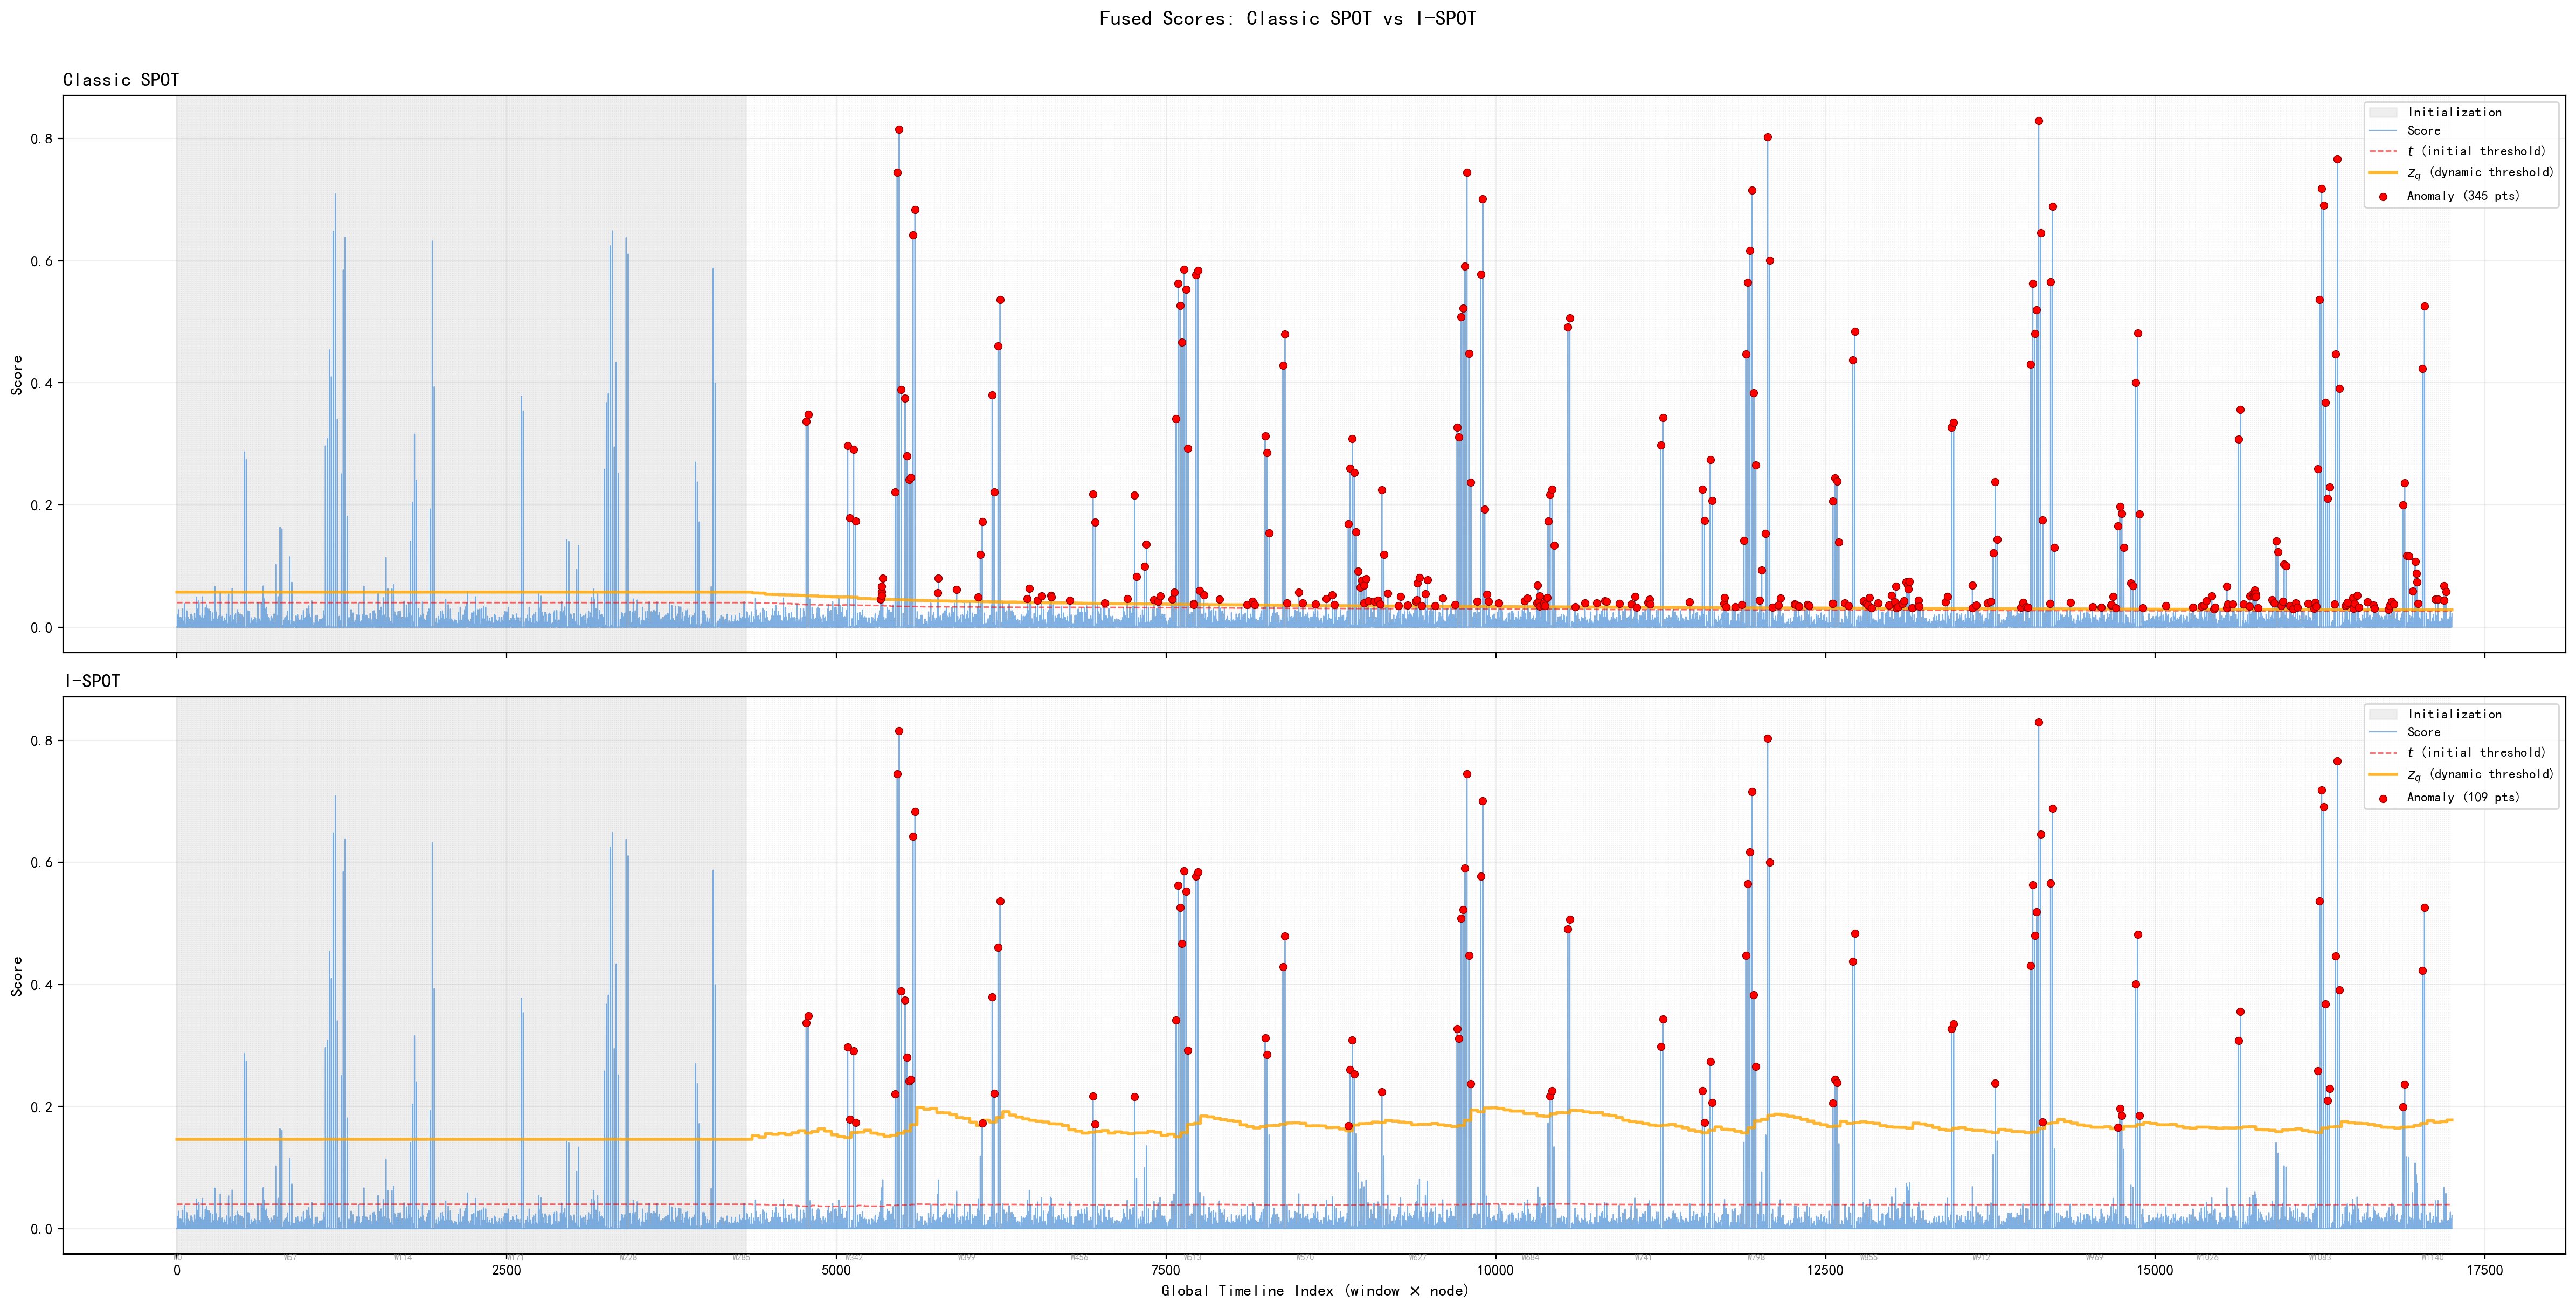
\includegraphics[width=\columnwidth]{../Tex/spot_vs_ispot_fused.png}
    \bicaption{融合分数上经典SPOT与I-SPOT检测结果对比}{Comparison of classic SPOT and I-SPOT on fused scores}
    \label{fig:spot_vs_ispot}
\end{figure}

上子图中经典SPOT的阈值呈单调下降趋势，后半段导致大量误报，根源在于排他性更新策略下的阈值衰减正反馈循环。下子图中I-SPOT的阈值始终保持平稳，检测标记仅出现在真实异常点附近，验证了包容性更新策略的有效性。


%=====================================================================
%  6 结论
%=====================================================================
\section{结论}

本文针对分布式集群中单指标多节点场景的异常检测问题，提出了CSAD-AT框架。主要贡献包括：（1）基于联通大数据生产环境构建了高质量的单指标多节点时序数据集；（2）设计了基于欧氏距离、自编码器嵌入和局部密度偏离的三种互补曲线相似性评分方法；（3）提出I-SPOT自适应阈值算法，通过包容性数据池更新与周期性GPD重估机制解决了经典SPOT的阈值衰减问题；（4）将上述组件整合为CSAD-AT框架，在无需人工阈值调整的条件下F1分数达到0.9864，显著优于现有方法。

未来工作将从两个方向拓展：一是将方法扩展至多指标联合检测场景，充分利用指标间的关联信息；二是在更多类型的分布式集群和监控指标上验证方法的泛化能力。

\section*{利益冲突声明}
所有作者声明不存在利益冲突关系。


%=====================================================================
%  参考文献
%=====================================================================
\begin{thebibliography}{99}

\bibitem{su2019omni}
Su Y, Zhao Y, Niu C, et al. Robust anomaly detection for multivariate time series through stochastic recurrent neural network[C]//Proceedings of the 25th ACM SIGKDD International Conference on Knowledge Discovery \& Data Mining. 2019: 2828--2837.

\bibitem{audibert2020usad}
Audibert J, Michiardi P, Guyard F, et al. USAD: unsupervised anomaly detection on multivariate time series[C]//Proceedings of the 26th ACM SIGKDD International Conference on Knowledge Discovery \& Data Mining. 2020: 3395--3404.

\bibitem{tuli2022tranad}
Tuli S, Casale G, Jennings N R. TranAD: deep transformer networks for anomaly detection in multivariate time series data[J]. Proceedings of the VLDB Endowment, 2022, 15(6): 1201--1214.

\bibitem{deng2021graph}
Deng A, Hooi B. Graph neural network-based anomaly detection in multivariate time series[C]//Proceedings of the AAAI Conference on Artificial Intelligence. 2021, 35(5): 4027--4035.

\bibitem{zhao2020mtadgat}
Zhao H, Wang Y, Duan J, et al. Multivariate time-series anomaly detection via graph attention network[C]//Proceedings of the IEEE International Conference on Data Mining. 2020: 841--850.

\bibitem{li2019madgan}
Li D, Chen D, Jin B, et al. MAD-GAN: multivariate anomaly detection for time series data with generative adversarial networks[C]//Proceedings of the International Conference on Artificial Neural Networks. 2019: 703--716.

\bibitem{siffer2017spot}
Siffer A, Fouque P A, Termier A, et al. Anomaly detection in streams with extreme value theory[C]//Proceedings of the 23rd ACM SIGKDD International Conference on Knowledge Discovery and Data Mining. 2017: 1067--1075.

\end{thebibliography}

\end{document}
% CSAD-AT 小论文 - 《数据与计算发展前沿》投稿格式
% 三线表 + 中英文双语标题
\documentclass[10.5pt,a4paper,twocolumn]{ctexart}

% ==================== 宏包 ====================
\usepackage[left=2cm,right=2cm,top=2.5cm,bottom=2.5cm]{geometry}
\usepackage{graphicx}
\usepackage{booktabs}       % 三线表
\usepackage{multirow}
\usepackage{amsmath,amssymb}
\usepackage{algorithm}
\usepackage{algorithmic}
\usepackage[hidelinks]{hyperref}
\usepackage{cite}
\usepackage{caption}
\usepackage{subcaption}
\usepackage{enumitem}
\usepackage{url}
\usepackage{xcolor}
\usepackage{float}

% ==================== 格式设置 ====================
\setlength{\columnsep}{0.7cm}
\renewcommand{\abstractname}{}
\CTEXsetup[format={\bfseries\zihao{4}}]{section}
\CTEXsetup[format={\bfseries\zihao{5}}]{subsection}
\CTEXsetup[format={\bfseries\zihao{5}}]{subsubsection}
\captionsetup{font=small,labelsep=space}
\captionsetup[table]{position=top}
\captionsetup[figure]{position=bottom}

% 图片路径
\graphicspath{{Img/}{Tex/}}

% ==================== 自定义双语标题命令 ====================
\newcommand{\bicaption}[2]{%
  \caption{#1\\{\small #2}}%
}

% ==================== 文档开始 ====================
\begin{document}

% ==================== 标题区（单栏） ====================
\twocolumn[
\begin{@twocolumnfalse}
\begin{center}

{\zihao{2}\bfseries CSAD-AT：面向分布式集群的阈值自适应\\单指标多节点异常检测框架\par}
\vspace{0.8em}

{\zihao{5} 杨婧雯$^{1}$，裴昌华$^{1*}$\par}
\vspace{0.3em}
{\zihao{6} 1.~中国科学院计算机网络信息中心，北京~~100190\par}
\vspace{1em}

% ---------- 中文摘要 ----------
\parbox{0.92\textwidth}{\zihao{5}
\textbf{摘\quad 要：}【目的】分布式集群中负载均衡类监控指标的正常波动具有随机性和不可预测性，传统基于历史模式学习的异常检测方法难以适用。同时，基于节点曲线相似性的检测方法对阈值参数高度敏感，难以在生产环境中直接部署。本文旨在提出一种无需人工阈值调优的端到端自适应异常检测框架。【方法】本文提出CSAD-AT（Curve Similarity-based Anomaly Detection with Adaptive Threshold）框架，融合欧氏距离、自编码器嵌入和局部密度偏离三种互补的曲线相似性评分方法，通过MinMax归一化与加权聚合统一多视角分数，并提出I-SPOT自适应阈值算法，采用包容性数据池更新与周期性GPD重估机制动态确定异常判定边界。【结果】在基于中国联通大数据生产环境构建的单指标多节点数据集上，CSAD-AT在无需人工阈值调整的条件下取得了0.9864的F1分数，优于三种曲线相似性方法在最优人工调参下的表现，且显著优于六种主流多元时序异常检测基线算法。【局限】当前实验仅在单一监控指标（RPC连接数）上验证，尚未扩展至多指标联合检测场景。【结论】基于节点曲线相似性的检测思路能够有效应对负载均衡类指标的随机波动挑战，I-SPOT自适应阈值算法成功消除了人工调参依赖，CSAD-AT框架具有良好的实际部署价值。
}
\vspace{0.4em}

\parbox{0.92\textwidth}{\zihao{5}
\textbf{关键词：}异常检测；分布式集群；曲线相似性；自适应阈值；极值理论
}
\vspace{1.2em}

% ---------- 英文标题 ----------
{\zihao{4}\bfseries CSAD-AT: A Threshold-Adaptive Single-Metric Multi-Node\\ Anomaly Detection Framework for Distributed Clusters\par}
\vspace{0.6em}
{\zihao{5} YANG Jingwen$^{1}$, PEI Changhua$^{1*}$\par}
\vspace{0.3em}
{\zihao{6} 1.~Computer Network Information Center, Chinese Academy of Sciences, Beijing 100190, China\par}
\vspace{0.8em}

% ---------- 英文摘要 ----------
\parbox{0.92\textwidth}{\zihao{5}
\textbf{Abstract:} [Objective] Load-balanced monitoring metrics in distributed clusters exhibit random and unpredictable normal fluctuations, making traditional history-based anomaly detection methods ineffective. While curve similarity-based methods show promise, their high sensitivity to threshold parameters hinders practical deployment. This paper proposes an end-to-end adaptive anomaly detection framework that eliminates manual threshold tuning. [Methods] We propose CSAD-AT (Curve Similarity-based Anomaly Detection with Adaptive Threshold), which integrates three complementary scoring methods based on Euclidean distance, autoencoder embedding, and local density deviation. Scores are unified through MinMax normalization and weighted aggregation. An improved I-SPOT adaptive threshold algorithm with inclusive data pool updates and periodic GPD re-estimation dynamically determines anomaly boundaries. [Results] On a single-metric multi-node dataset from China Unicom production environments, CSAD-AT achieves an F1 score of 0.9864 without manual threshold tuning, outperforming all three similarity methods under optimal manual tuning and significantly surpassing six state-of-the-art baselines. [Limitations] Experiments are currently limited to a single monitoring metric (RPC connection count). [Conclusions] Curve similarity-based detection effectively addresses the challenge of random fluctuations in load-balanced metrics. The I-SPOT algorithm successfully eliminates manual parameter tuning dependency.
}
\vspace{0.4em}

\parbox{0.92\textwidth}{\zihao{5}
\textbf{Keywords:} anomaly detection; distributed cluster; curve similarity; adaptive threshold; extreme value theory
}
\vspace{1.5em}
\end{center}
\end{@twocolumnfalse}
]


%=====================================================================
%  引言
%=====================================================================
\section{引言}

随着云计算和大数据技术的快速发展，分布式集群已成为支撑大规模数据处理与计算服务的核心基础设施。在企业级生产环境中，分布式集群通常由数十至数百个计算节点组成，通过YARN（Yet Another Resource Negotiator）等资源调度框架实现计算资源的统一管理与动态分配。集群中各节点的运行状态由Prometheus等监控系统持续采集，形成海量的多节点时间序列监控数据。及时准确地从这些监控数据中检测出异常节点，对于保障服务质量、降低运维成本具有重要意义。

然而，分布式集群环境中的异常检测面临独特的技术挑战。以RPC连接数等与用户负载强相关的监控指标为例，其正常波动具有随机性和不可预测性，难以通过先验知识定义统一的正常模式。传统的单节点历史模式学习方法（如基于重构的自编码器、基于预测的Transformer等）在面对此类指标时，往往因无法建立稳定的正常基线而导致高误报率或高漏报率。

值得注意的是，在负载均衡机制的作用下，分布式集群中正常运行的各节点承担相近的工作负载，其同一监控指标的时序曲线呈现出高度的形态相似性。当个别节点发生故障时，其曲线会显著偏离群体模式，形成可识别的"离群曲线"。这一"正常聚集、异常离群"的数据特性为异常检测提供了新思路：通过度量节点间曲线的差异程度来识别偏离群体行为的异常节点。

基于曲线相似性的方法虽然在理论上具有优势，但在实际部署中面临一个核心难题：检测阈值的选择。实验表明，此类方法的最优参数处于极窄的有效区间内，细微的阈值偏移便可导致性能骤变，呈现显著的"悬崖效应"。由于不同集群的节点数量、负载模式、指标量纲等因素各异，在一个集群上调优的参数难以直接迁移，而获取高质量标注数据用于参数调优的成本又极为高昂。因此，如何实现阈值的动态自适应调整，成为将基于曲线相似性的方法推向实际应用的关键技术瓶颈。

针对上述挑战，本文提出CSAD-AT（Curve Similarity-based Anomaly Detection with Adaptive Threshold）框架。该框架融合欧氏距离、自编码器嵌入和局部密度偏离三种互补的曲线相似性评分方法，通过MinMax归一化与加权聚合实现多视角分数融合，并提出I-SPOT（Inclusive SPOT）自适应阈值算法，基于极值理论动态确定异常判定边界，实现端到端的无人工调参异常检测。在基于联通大数据生产环境构建的数据集上，CSAD-AT取得了0.9864的F1分数，显著优于现有基线方法。


%=====================================================================
%  1 相关工作
%=====================================================================
\section{相关工作}

时间序列异常检测是智能运维（AIOps）领域的核心任务之一。现有方法主要包括基于统计的方法、基于机器学习的方法和基于深度学习的方法三大类。

在基于深度学习的方法中，OmniAnomaly\cite{su2019omni}采用随机变分自编码器学习多元时间序列的正常分布，通过重构概率识别异常。USAD\cite{audibert2020usad}在自编码器基础上引入对抗训练增强鲁棒性。TranAD\cite{tuli2022tranad}基于Transformer架构并结合对抗训练提升异常敏感度。GDN\cite{deng2021graph}通过图神经网络建模变量间拓扑关系。MTAD-GAT\cite{zhao2020mtadgat}结合图注意力网络和时间卷积网络同时建模变量间关联和时间依赖。MAD-GAN\cite{li2019madgan}采用LSTM构建生成对抗网络学习正常数据分布。

上述方法主要面向多变量间的关联异常设计，对分布式集群中单指标多节点的场景缺乏针对性。在自适应阈值方面，SPOT算法\cite{siffer2017spot}基于极值理论对流数据进行动态阈值检测，但其排他性更新策略在概念漂移条件下存在阈值衰减问题。本文提出的CSAD-AT框架融合多视角曲线相似性评分与改进的I-SPOT自适应阈值算法，实现端到端的无人工调参异常检测。


%=====================================================================
%  2 数据集构建
%=====================================================================
\section{数据集构建}

\subsection{数据来源与采集}

本研究的数据来源于中国联通大数据生产底座平台。该平台采用YARN架构进行分布式计算资源的统一调度与管理，其核心架构如图\ref{fig:yarn_arch}所示。ResourceManager作为集群的中央调度器，通过RPC Router接收各NodeManager的心跳与资源请求；各NodeManager负责本地容器的生命周期管理，通过RPC Client与ResourceManager保持通信；Prometheus监控系统实时采集各节点的运行指标。

\begin{figure}[htbp]
    \centering
    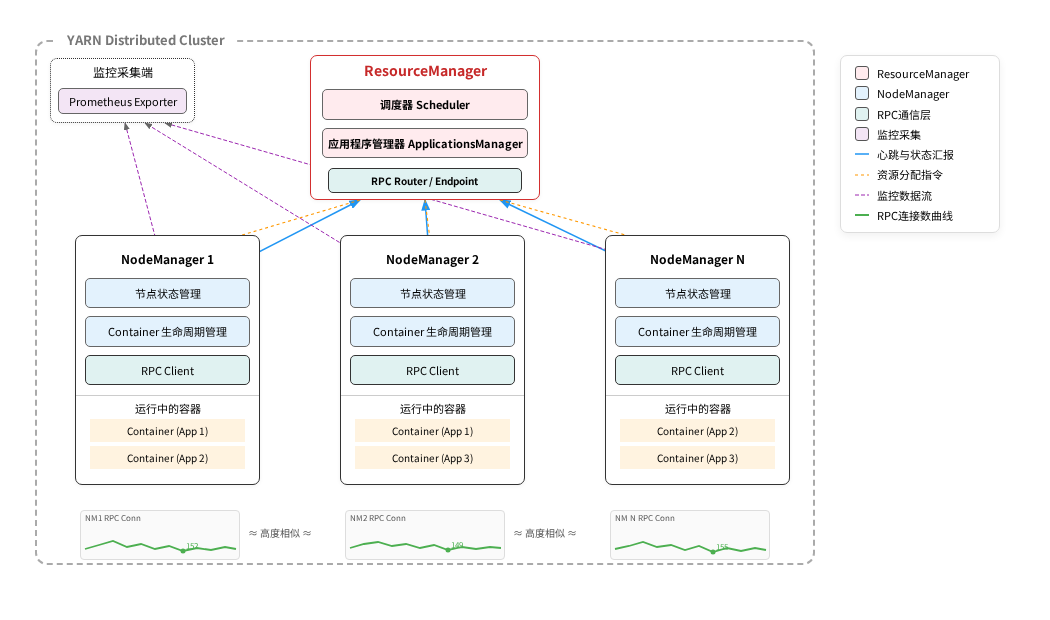
\includegraphics[width=\columnwidth]{yarn_arch.png}
    \bicaption{YARN分布式集群架构与RPC Router连接数指标示意}{YARN cluster architecture and RPC Router connection count}
    \label{fig:yarn_arch}
\end{figure}

在长期运维实践中发现，与用户负载强相关的监控指标（如RPC连接数）呈现出独特的统计特性：正常波动模式难以通过先验知识统一定义，且随全局负载呈现不可预测的剧烈变化。然而，得益于负载均衡机制的作用，正常运行状态下各节点同一指标的时序曲线呈现出高度的形态相似性。本研究选取RPC Router连接数作为核心研究指标，通过Prometheus API接口采集了多个生产集群在连续运行周期内所有节点的该指标时序数据，形成训练集（覆盖30天连续运行数据）和测试集（覆盖8天连续运行数据），原始数据采样间隔为60秒。

\subsection{数据集预处理与标注}

为构建适用于算法研究的高质量数据集，本研究对原始监控时序数据实施了系统化的预处理与半人工标注流程，整体流程如图\ref{fig:annotation_flow}所示。预处理阶段执行三项操作：（1）线性插值填充短暂缺失值；（2）将所有节点数据对齐至统一的60秒间隔时间戳；（3）剔除长时间段数据完全缺失的节点记录。

\begin{figure}[htbp]
    \centering
    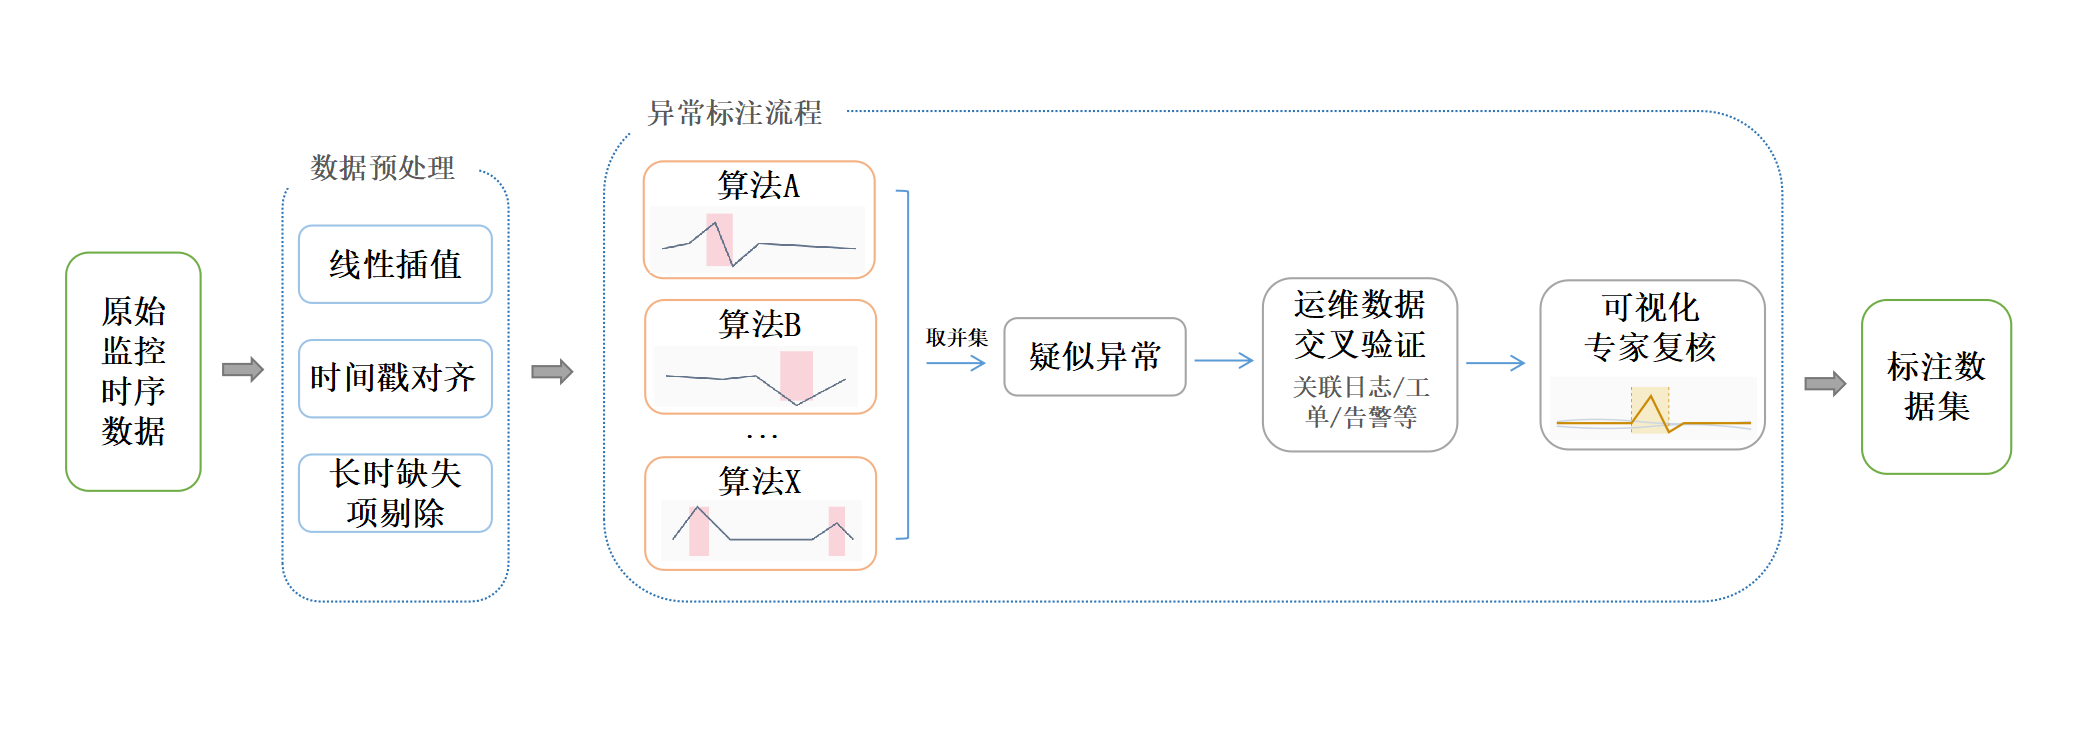
\includegraphics[width=\columnwidth]{draft/annotation_flow_new.png}
    \bicaption{数据集预处理与半人工标注流程}{Dataset preprocessing and semi-manual annotation workflow}
    \label{fig:annotation_flow}
\end{figure}

在异常标注阶段，采用多算法初筛与专家判读相结合的半人工标注策略。首先利用多种无监督离群点检测算法以宽松阈值筛选疑似异常片段；然后关联查询对应节点的运维日志、工单记录等多源数据进行交叉验证；最终由具备丰富运维经验的专家结合可视化工具做出异常判定。

\subsection{数据集统计与可视化}

经过预处理与标注，构建了适用于分布式集群节点级异常检测的单指标多节点时间序列数据集，详细统计信息如表\ref{tab:dataset_stats}所示。

\begin{table}[htbp]
    \centering
    \bicaption{数据集统计数据}{Dataset statistics}
    \label{tab:dataset_stats}
    \begin{tabular}{lccccc}
        \toprule
         & 节点数 & 数据点 & 异常段 & 异常点 & 异常比例 \\
        \midrule
        训练集   & 30 & 86400 & /  & /    & /      \\
        测试集A  & 15 & 11520 & 72 & 901  & 7.82\% \\
        测试集B  & 15 & 11520 & 33 & 907  & 7.87\% \\
        测试集   & 30 & 23040 & 105& 1808 & 7.85\% \\
        \bottomrule
    \end{tabular}
\end{table}

该数据集的核心特征在于直观揭示了分布式集群在负载均衡机制下的运行规律，如图\ref{fig:anomaly_curve}所示。在绝大部分时间内，集群内多数节点的监控指标曲线呈现高度的形态同步性与数值聚集性，形成清晰的"正常行为簇"。当个别节点发生故障时，其曲线显著偏离共同的"行为簇"，表现为"离群曲线"。

\begin{figure}[htbp]
    \centering
    
\includegraphics[width=\columnwidth]{dataset_anomaly_example.png}
    \bicaption{测试集A典型异常片段时序可视化（红色曲线为异常节点，粉色阴影为异常时段）}{Visualization of typical anomaly segments in Test Set A}
    \label{fig:anomaly_curve}
\end{figure}


%=====================================================================
%  3 基于曲线相似性的异常评分方法
%=====================================================================
\section{基于曲线相似性的异常评分方法}

本节从数值距离、嵌入空间距离和局部密度三个互补视角设计异常评分方法。三种方法的核心思想一致：通过度量节点间曲线的偏离程度量化异常可能性。

\subsection{基于欧氏距离的数值相似性度量}\label{subsec:euclidean}

给定包含$N$个节点的分布式集群，每个节点$i$在时刻$t$的监控指标观测值记为$x_i^t$。采用滑动窗口机制对原始序列进行分段处理，对于长度为$w$的时间窗口，节点$i$在时刻$t$的窗口序列表示为$\mathbf{x}_i^t = [x_i^{t-w+1}, \ldots, x_i^t]^T \in \mathbb{R}^w$。节点$i$与节点$j$在时刻$t$的欧氏距离定义为：
\begin{equation}
    d_{ij}^t = \|\mathbf{x}_i^t - \mathbf{x}_j^t\|_2 = \sqrt{\sum_{k=t-w+1}^{t}(x_i^k - x_j^k)^2}
\end{equation}

计算所有节点两两之间的欧氏距离构成距离矩阵$\mathbf{D}^t \in \mathbb{R}^{N \times N}$，计算均值$\mu_t$和标准差$\sigma_t$。对每个节点$i$，计算其与其他所有节点的平均距离：
\begin{equation}
    \bar{d}_i^t = \frac{1}{N-1}\sum_{j=1, j \neq i}^{N} d_{ij}^t
\end{equation}

节点$i$的异常分数采用Z-score标准化形式：
\begin{equation}\label{eq:euc_score}
    s_i^t = \frac{\bar{d}_i^t - \mu_t}{\sigma_t}
\end{equation}

设定阈值$T$，若$s_i^t > T$则判定节点$i$在时刻$t$异常。

\subsection{基于自编码器嵌入的形态相似性度量}

欧氏距离方法对曲线绝对数值高度敏感，可能忽略形态层面的相似性。为克服此局限，引入自编码器进行深度特征提取，其网络结构如图\ref{fig:autoencoder}所示。

\begin{figure}[htbp]
    \centering
    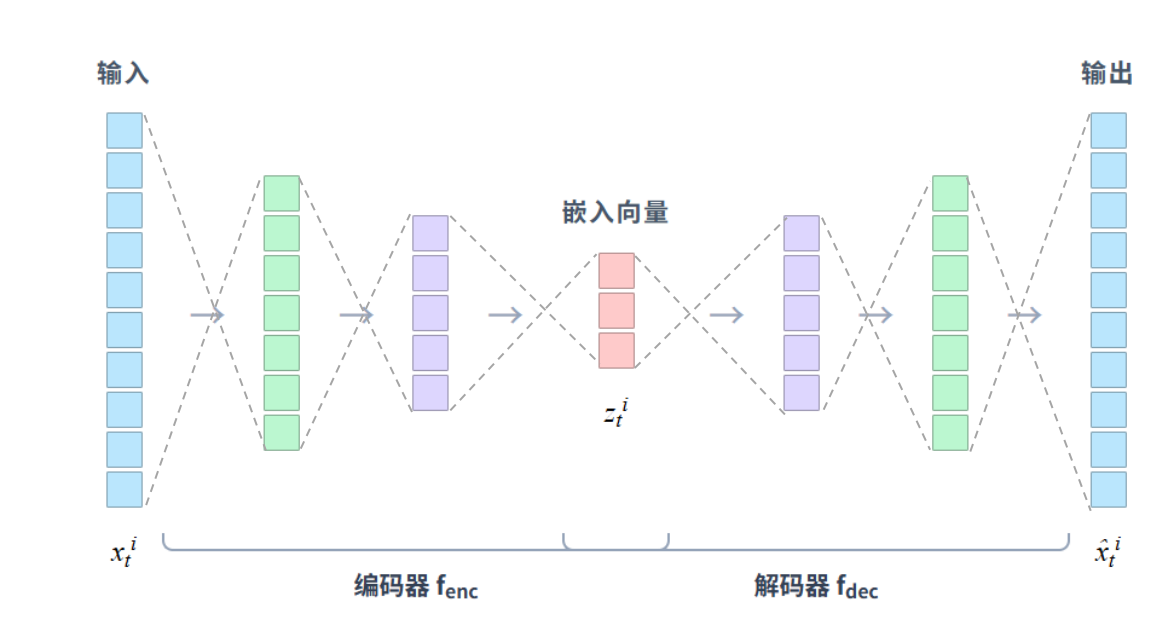
\includegraphics[width=0.85\columnwidth]{draft/autoencoder_arch.png}
    \bicaption{自编码器网络结构示意图}{Architecture of the autoencoder network}
    \label{fig:autoencoder}
\end{figure}

编码器$f_{\text{enc}}$通过多层全连接网络将输入序列$\mathbf{x}_i^t$压缩为低维嵌入向量$\mathbf{z}_i^t = f_{\text{enc}}(\mathbf{x}_i^t)$，解码器$f_{\text{dec}}$以对称结构重构原始输入$\hat{\mathbf{x}}_i^t = f_{\text{dec}}(\mathbf{z}_i^t)$。通过最小化均方误差训练，嵌入向量保留曲线最本质的形态特征。网络包含三层全连接编码器（维度$w \to 128 \to 128 \to 5$）和对称的三层解码器，隐藏层采用ReLU激活函数，Adam优化器，学习率0.001，训练50个epoch。应用阶段仅使用编码器，基于嵌入向量计算节点间距离$d_{ij}^t = \|\mathbf{z}_i^t - \mathbf{z}_j^t\|_2$，后续异常分数计算与欧氏距离方法一致。

\subsection{基于局部密度的偏离评分}\label{subsec:density}

借鉴局部离群因子（LOF）的思想，设计基于$k$近邻可达密度的连续异常评分方法。对每个时间窗口内的每个节点$i$，基于距离矩阵找到其$k_{\text{nn}}$个最近邻节点，计算局部可达密度：
\begin{equation}
    \text{LRD}_i = \frac{1}{\frac{1}{|\mathcal{N}_i|}\sum_{j \in \mathcal{N}_i} d_{ij} + \epsilon}
\end{equation}
其中$\mathcal{N}_i$为节点$i$的邻域集合，$\epsilon$为防止除零的小常数。密度偏离分数通过三个子分数的加权组合得到：
\begin{equation}\label{eq:density_score}
    s_i^t = w_1 \cdot z_{\text{LRD}} + w_2 \cdot z_{k\text{th}} + w_3 \cdot z_{\text{nbr}}
\end{equation}
其中$z_{\text{LRD}}$、$z_{k\text{th}}$、$z_{\text{nbr}}$分别为LRD、第$k$近邻距离和邻居数量的Z-score标准化值。

\subsection{参数敏感性分析}\label{subsec:sensitivity}

在构建的数据集上进行实验评估，三种方法在最优参数下的检测结果如表\ref{tab:baseline_results}所示，F1分数均超过0.96，显著优于现有基线算法。

\begin{table*}[htbp]
    \centering
    \bicaption{基线算法与曲线相似性方法异常检测结果}{Anomaly detection results of baseline algorithms and curve similarity methods}
    \label{tab:baseline_results}
    \begin{tabular}{llccc}
        \toprule
        类别 & 算法 & Precision & Recall & F1 \\
        \midrule
        \multirow{6}{*}{基线算法}
        & TranAD\cite{tuli2022tranad}         & 0.8889 & 0.3932 & 0.5452 \\
        & USAD\cite{audibert2020usad}          & 0.6892 & 0.5567 & 0.6159 \\
        & OmniAnomaly\cite{su2019omni}         & 0.6054 & 0.4593 & 0.5224 \\
        & GDN\cite{deng2021graph}              & 0.3101 & 0.5218 & 0.3890 \\
        & MAD-GAN\cite{li2019madgan}           & 0.6309 & 0.6309 & 0.6891 \\
        & MTAD-GAT\cite{zhao2020mtadgat}       & 0.3492 & 0.1573 & 0.2169 \\
        \midrule
        \multirow{3}{*}{\shortstack{相似性方法\\（最优阈值）}}
        & 欧氏距离     & 0.9826 & 0.9657 & \underline{0.9741} \\
        & 自编码器嵌入 & 0.9792 & 0.9592 & 0.9691 \\
        & 密度偏离     & 0.9605 & 0.9659 & 0.9632 \\
        \bottomrule
    \end{tabular}
\end{table*}

然而，上述优异性能严重依赖精确的参数调优。图\ref{fig:threshold_sensitivity}展示了三种方法的F1分数随阈值变化的趋势，均呈现"先升后降"特征，且在最优阈值附近存在陡峭的性能衰减，呈现显著的"悬崖效应"。这揭示了基于曲线相似性方法在实际部署中面临的核心挑战：高性能严重依赖参数调优，而参数难以跨场景复用。

\begin{figure}[htbp]
    \centering
    
\includegraphics[width=\columnwidth]{draft/threshold_sensitivity.png}
    \bicaption{三种检测方法在不同窗口大小下F1分数随阈值变化的折线图}{F1 score vs.\ threshold for three detection methods under different window sizes}
    \label{fig:threshold_sensitivity}
\end{figure}


%=====================================================================
%  4 CSAD-AT框架
%=====================================================================
\section{CSAD-AT框架}

\subsection{框架概述}

为解决阈值依赖问题，本文提出CSAD-AT框架，其整体架构如图\ref{fig:csad_framework}所示。框架包含三个核心模块：（1）多视角相似性评分模块；（2）分数归一化与聚合模块；（3）I-SPOT自适应阈值检测模块。

\begin{figure*}[htbp]
    \centering
    
\includegraphics[width=0.95\textwidth]{image4-6.png}
    \bicaption{CSAD-AT框架整体架构}{Overall architecture of the CSAD-AT framework}
    \label{fig:csad_framework}
\end{figure*}

\subsection{分数归一化与聚合}

三种评分方法输出的原始分数在量纲和数值范围上存在显著差异。CSAD-AT框架对每种方法的分数序列执行两步归一化。

第一步，负值截断：
\begin{equation}
    s'^{(m)} = \max(s^{(m)}, 0)
\end{equation}

第二步，MinMax归一化：
\begin{equation}
    \tilde{s}^{(m)} = \frac{s'^{(m)} - s'^{(m)}_{\min}}{s'^{(m)}_{\max} - s'^{(m)}_{\min}}
\end{equation}

归一化后通过加权平均聚合：
\begin{equation}
    s_{\text{fused}} = \sum_{m=1}^{M} w_m \cdot \tilde{s}^{(m)}, \quad \sum_{m=1}^{M} w_m = 1
\end{equation}
其中$M=3$，默认等权$w_1 = w_2 = w_3 = 1/3$。选择加权平均策略的理由在于：相比最大值融合保留连续分数信息，相比投票机制输出连续值有利于GPD尾部建模。

\subsection{I-SPOT自适应阈值算法}\label{subsec:ispot}

经典SPOT\cite{siffer2017spot}算法利用广义帕累托分布（GPD）对分数分布尾部建模。给定异常分数序列，选取初始阈值$t_0$，超额值$Y = S - t_0$（$S > t_0$）的条件分布近似为GPD：
\begin{equation}
    G_{\xi,\sigma}(y) = 1 - \left(1 + \frac{\xi y}{\sigma}\right)^{-1/\xi}, \quad y > 0
\end{equation}

对于给定风险水平$q$，异常检测阈值为：
\begin{equation}\label{eq:spot_threshold}
    z_q = t_0 + \frac{\hat{\sigma}}{\hat{\xi}}\left[\left(\frac{n}{N_t} \cdot q\right)^{-\hat{\xi}} - 1\right]
\end{equation}

经典SPOT仅将未超过阈值的正常数据纳入更新池，在概念漂移场景下引发阈值衰减问题。本文提出I-SPOT算法，采用包容性更新策略。维护最大容量$W_{\max}$的FIFO数据池$\mathcal{D}_t$：
\begin{equation}
    \mathcal{D}_{t+1} = \begin{cases}
        \mathcal{D}_t \cup \{s_t\}, & \text{if } |\mathcal{D}_t| < W_{\max} \\
        (\mathcal{D}_t \setminus \{s_{\text{oldest}}\}) \cup \{s_t\}, & \text{otherwise}
    \end{cases}
\end{equation}

所有数据点均纳入数据池，每隔$T_{\text{update}}$步重新拟合GPD参数并更新阈值。算法完整流程如算法\ref{alg:ispot}所示。

\begin{algorithm}[htbp]
\caption{I-SPOT自适应阈值算法}
\label{alg:ispot}
\begin{algorithmic}[1]
\REQUIRE 分数流$\{s_1, s_2, \ldots\}$，风险水平$q$，分位数$\textit{level}$，池容量$W_{\max}$，重估间隔$T_{\text{update}}$，初始长度$n_0$
\ENSURE 异常判定结果，阈值序列$\{z_q^{(t)}\}$
\STATE $\mathcal{D} \gets \{s_1, \ldots, s_{n_0}\}$；$t_0 \gets \text{Percentile}(\mathcal{D}, \textit{level})$
\STATE $(\hat{\xi}, \hat{\sigma}) \gets \text{GrimshawMLE}(\{s\!-\!t_0 \mid s \in \mathcal{D}, s > t_0\})$
\STATE $z_q \gets \text{Threshold}(t_0, \hat{\xi}, \hat{\sigma}, q)$；$\textit{steps} \gets 0$
\FOR{\textbf{each} $s_t$}
    \IF{$s_t > z_q$}
        \STATE 标记时刻$t$为异常
    \ENDIF
    \IF{$|\mathcal{D}| \geq W_{\max}$}
        \STATE $\mathcal{D} \gets \mathcal{D} \setminus \{s_{\text{oldest}}\}$
    \ENDIF
    \STATE $\mathcal{D} \gets \mathcal{D} \cup \{s_t\}$；$\textit{steps} \gets \textit{steps} + 1$
    \IF{$\textit{steps} \geq T_{\text{update}}$}
        \STATE 重新拟合GPD并更新$z_q$；$\textit{steps} \gets 0$
    \ENDIF
\ENDFOR
\end{algorithmic}
\end{algorithm}

CSAD-AT将所有节点的聚合分数按窗口交织为全局时间序列$\mathbf{S}_{\text{global}}$，在其上运行单个I-SPOT实例。该设计使所有节点共享同一阈值，降低计算开销，且全局序列样本量更大使GPD拟合更稳健。


%=====================================================================
%  5 实验验证与分析
%=====================================================================
\section{实验验证与分析}

\subsection{实验设置}

实验在本文构建的数据集上进行，评估指标采用精确率（Precision）、召回率（Recall）和F1分数。I-SPOT超参数：$q = 0.0065$，$\text{level} = 0.98$，$T_{\text{update}} = 50$，$n_0 = 1500$。基线算法包括TranAD、USAD、OmniAnomaly、GDN、MAD-GAN和MTAD-GAT六种主流方法，均使用开源代码和默认参数。

\subsection{整体性能分析}

表\ref{tab:overall_results}展示了CSAD-AT与各对比方法的性能。

\begin{table}[htbp]
    \centering
    \bicaption{CSAD-AT整体性能对比}{Overall performance comparison of CSAD-AT}
    \label{tab:overall_results}
    \begin{tabular}{lccc}
        \toprule
        算法 & Precision & Recall & F1 \\
        \midrule
        TranAD\cite{tuli2022tranad}      & 0.8889 & 0.3932 & 0.5452 \\
        USAD\cite{audibert2020usad}       & 0.6892 & 0.5567 & 0.6159 \\
        OmniAnomaly\cite{su2019omni}      & 0.6054 & 0.4593 & 0.5224 \\
        GDN\cite{deng2021graph}           & 0.3101 & 0.5218 & 0.3890 \\
        MAD-GAN\cite{li2019madgan}        & 0.6309 & 0.6309 & 0.6891 \\
        MTAD-GAT\cite{zhao2020mtadgat}    & 0.3492 & 0.1573 & 0.2169 \\
        \midrule
        欧氏距离（最优阈值）     & 0.9826 & 0.9657 & \underline{0.9741} \\
        自编码器嵌入（最优阈值） & 0.9792 & 0.9592 & 0.9691 \\
        密度偏离（最优阈值）     & 0.9605 & 0.9659 & 0.9632 \\
        \midrule
        \textbf{CSAD-AT}        & \textbf{1.0000} & 0.9732 & \textbf{0.9864} \\
        \bottomrule
    \end{tabular}
\end{table}

CSAD-AT在无需人工阈值调整的条件下F1分数达到0.9864，优于各评分方法在最优阈值下的性能，且显著优于所有基线算法，证明分数聚合与I-SPOT自适应阈值能够有效替代人工调参。

\subsection{分数聚合策略对比}

表\ref{tab:agg_compare}对比了不同归一化与聚合策略的组合。

\begin{table}[htbp]
    \centering
    \bicaption{不同分数聚合策略的性能对比}{Performance comparison of different score aggregation strategies}
    \label{tab:agg_compare}
    \begin{tabular}{ccccc}
        \toprule
        归一化 & 聚合策略 & Precision & Recall & F1 \\
        \midrule
        Z-score & 加权平均 & 0.9157 & 0.9806 & 0.9470 \\
        MinMax  & 最大值   & 1.0000 & 0.8426 & 0.9146 \\
        MinMax  & 投票     & 0.9831 & 0.9587 & \underline{0.9707} \\
        MinMax  & 加权平均 & 1.0000 & 0.9732 & \textbf{0.9864} \\
        \bottomrule
    \end{tabular}
\end{table}

MinMax归一化在所有聚合策略下均优于Z-score归一化。MinMax加权平均以0.9864的F1分数取得最优性能，投票策略居次（0.9707），最大值策略最低（0.9146）。

\subsection{消融实验}

表\ref{tab:ablation}展示了各评分方法单独与I-SPOT结合的性能。

\begin{table}[htbp]
    \centering
    \bicaption{消融实验：各评分方法与I-SPOT结合的性能}{Ablation study: each scoring method combined with I-SPOT}
    \label{tab:ablation}
    \begin{tabular}{lccc}
        \toprule
        检测配置 & Precision & Recall & F1 \\
        \midrule
        欧氏距离 + I-SPOT     & 1.0000 & 0.9187 & \underline{0.9576} \\
        自编码器嵌入 + I-SPOT  & 0.9891 & 0.8667 & 0.9239 \\
        密度偏离 + I-SPOT      & 1.0000 & 0.8917 & 0.9427 \\
        \midrule
        CSAD-AT（三种融合）    & 1.0000 & 0.9732 & \textbf{0.9864} \\
        \bottomrule
    \end{tabular}
\end{table}

完整的三方法融合方案F1达到0.9864，显著优于单一方法。召回率从0.9187提升至0.9732，说明三种方法形成有效互补：欧氏距离捕捉数值偏离，自编码器嵌入识别形态异常，密度偏离发现孤立型异常。

\subsection{I-SPOT与经典SPOT对比}

表\ref{tab:spot_compare}对比了两种算法在相同超参数下的性能。

\begin{table}[htbp]
    \centering
    \bicaption{经典SPOT与I-SPOT性能对比}{Performance comparison of classic SPOT and I-SPOT}
    \label{tab:spot_compare}
    \begin{tabular}{lccc}
        \toprule
        阈值算法 & Precision & Recall & F1 \\
        \midrule
        经典SPOT & 0.3218 & 1.0000 & 0.4870 \\
        I-SPOT   & 1.0000 & 0.9732 & \textbf{0.9864} \\
        \bottomrule
    \end{tabular}
\end{table}

经典SPOT精确率仅0.3218，超过三分之二的报警为误报；I-SPOT实现了1.0的精确率，F1提升约50个百分点。图\ref{fig:spot_vs_ispot}直观展示了两者的差异。

\begin{figure}[htbp]
    \centering
    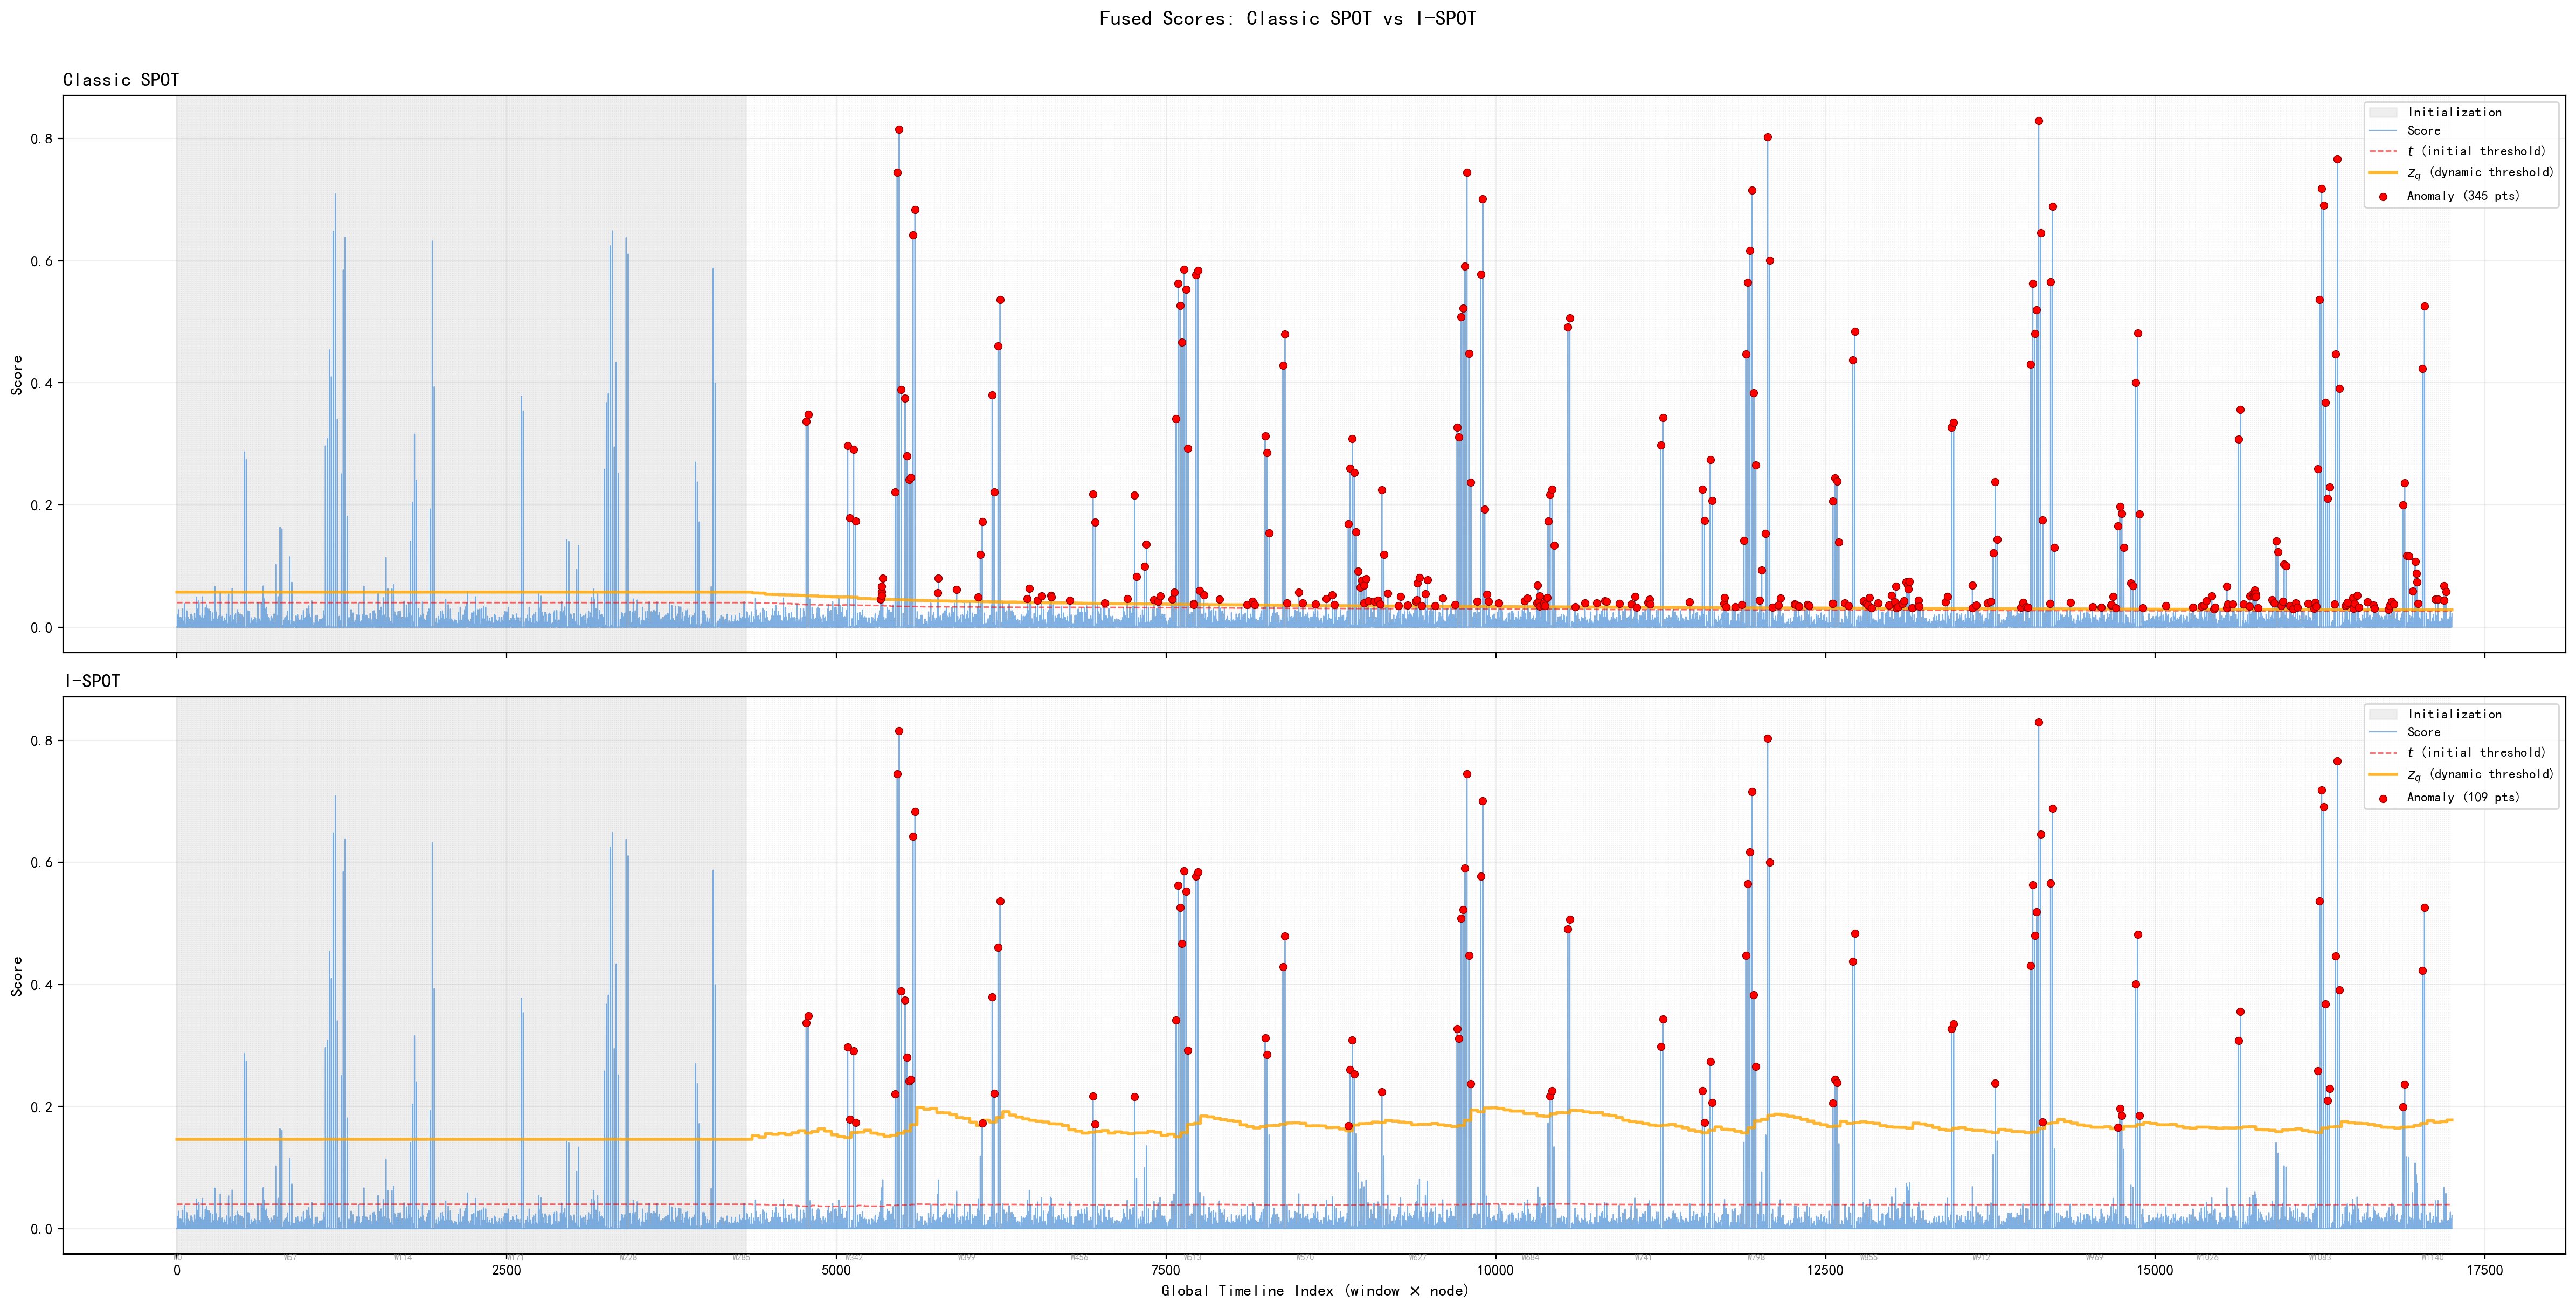
\includegraphics[width=\columnwidth]{../Tex/spot_vs_ispot_fused.png}
    \bicaption{融合分数上经典SPOT与I-SPOT检测结果对比}{Comparison of classic SPOT and I-SPOT on fused scores}
    \label{fig:spot_vs_ispot}
\end{figure}

上子图中经典SPOT的阈值呈单调下降趋势，后半段导致大量误报，根源在于排他性更新策略下的阈值衰减正反馈循环。下子图中I-SPOT的阈值始终保持平稳，检测标记仅出现在真实异常点附近，验证了包容性更新策略的有效性。


%=====================================================================
%  6 结论
%=====================================================================
\section{结论}

本文针对分布式集群中单指标多节点场景的异常检测问题，提出了CSAD-AT框架。主要贡献包括：（1）基于联通大数据生产环境构建了高质量的单指标多节点时序数据集；（2）设计了基于欧氏距离、自编码器嵌入和局部密度偏离的三种互补曲线相似性评分方法；（3）提出I-SPOT自适应阈值算法，通过包容性数据池更新与周期性GPD重估机制解决了经典SPOT的阈值衰减问题；（4）将上述组件整合为CSAD-AT框架，在无需人工阈值调整的条件下F1分数达到0.9864，显著优于现有方法。

未来工作将从两个方向拓展：一是将方法扩展至多指标联合检测场景，充分利用指标间的关联信息；二是在更多类型的分布式集群和监控指标上验证方法的泛化能力。

\section*{利益冲突声明}
所有作者声明不存在利益冲突关系。


%=====================================================================
%  参考文献
%=====================================================================
\begin{thebibliography}{99}

\bibitem{su2019omni}
Su Y, Zhao Y, Niu C, et al. Robust anomaly detection for multivariate time series through stochastic recurrent neural network[C]//Proceedings of the 25th ACM SIGKDD International Conference on Knowledge Discovery \& Data Mining. 2019: 2828--2837.

\bibitem{audibert2020usad}
Audibert J, Michiardi P, Guyard F, et al. USAD: unsupervised anomaly detection on multivariate time series[C]//Proceedings of the 26th ACM SIGKDD International Conference on Knowledge Discovery \& Data Mining. 2020: 3395--3404.

\bibitem{tuli2022tranad}
Tuli S, Casale G, Jennings N R. TranAD: deep transformer networks for anomaly detection in multivariate time series data[J]. Proceedings of the VLDB Endowment, 2022, 15(6): 1201--1214.

\bibitem{deng2021graph}
Deng A, Hooi B. Graph neural network-based anomaly detection in multivariate time series[C]//Proceedings of the AAAI Conference on Artificial Intelligence. 2021, 35(5): 4027--4035.

\bibitem{zhao2020mtadgat}
Zhao H, Wang Y, Duan J, et al. Multivariate time-series anomaly detection via graph attention network[C]//Proceedings of the IEEE International Conference on Data Mining. 2020: 841--850.

\bibitem{li2019madgan}
Li D, Chen D, Jin B, et al. MAD-GAN: multivariate anomaly detection for time series data with generative adversarial networks[C]//Proceedings of the International Conference on Artificial Neural Networks. 2019: 703--716.

\bibitem{siffer2017spot}
Siffer A, Fouque P A, Termier A, et al. Anomaly detection in streams with extreme value theory[C]//Proceedings of the 23rd ACM SIGKDD International Conference on Knowledge Discovery and Data Mining. 2017: 1067--1075.

\end{thebibliography}

\end{document}
